% \renewcommand{\includegraphics}[2][]{\texttt{FIGURE}}

Our aim will be to calculate the reflection from certain types of radial quantum tree graph that have an infinite number of generations yet finite depth.  Recall that a radial quantum tree graph is characterized by that every property of the graph depends only on the radial distance to the root of the tree, specifically all edges in the same generation have the same length and all vertices in the same generation have the same branching number. This gives rise to a rotational symmetry: the graph is invariant under discrete rotation (more specifically permutation, see section \ref{sec: graph symmetries}) of edges in the same generation around each branching point. This symmetry will be exploited to collapse the radial quantum tree graph with standard matching conditions to a quantum graph consisting of joined intervals with special matching conditions at the vertices, as a means of better understanding scattering properties of the graph.


\section{Preliminaries}

A quantum snowflake graph $\Gamma$ is a radial quantum tree (cf.\ definition \ref{def: radial quantum tree graph}) with infinite number of generations in which the branching number $m$ is the same for each generation, giving $m^k$ edges in the $k$:th generation. Furthermore the length of all edges in generation $k$ is $\ell_0\beta^k$ where $\beta$ is some constant. If $\beta<1$ the graph has a finite depth $\sum_{k=0}^{\infty} \ell_0\beta^k = \frac{\ell_0}{1-\beta}$. The `volume' of the graph, being the total edge length, given by $\sum_{k=0}^{\infty} \ell_0(m\beta)^k$, is finite only if in addition $m\beta < 1$, which is not the case in general.

Note that if the number of generations is finite and all edges are finite, then the entire incoming wave will necessarily get reflected, $|R| = 1$. However, if the number of generations is infinite, this is no longer necessarily the case and $|R|$ may be less than 1, the wave can disperse into the infinite structure of edges, never being reflected. Note that we are considering snowflake graphs with standard matching conditions at each vertex.

\begin{figure}[!h]
  \centering
  \includegraphics[width=0.8\textwidth]{img/snowflake_2.tikz}
  \caption{A snowflake with only 2 generations, branching number $m=4$ and $\beta < 1$, illustrating our notation.}
  \label{fig: snowflake notation}
\end{figure}

We begin by extending the notation introduced for radial quantum trees in definition~\ref{def: radial quantum tree graph}. With figure~\ref{fig: snowflake notation} in mind, edges are indexed by $e_{j_1,j_2,\ldots,j_n} = e_{\vec{j}}$ with $1 \le j_k \le m$ for $1 \le k \le n$. The $n$:th generation of edges is the set of edges $e_{\vec{j}}$ such that $\vec{j}$ contains $n$ elements, with the exception $e_0$ belonging to the 0:th generation. Similarly, the vertex $v_{\vec{j}}$ is the vertex where the right end-point of the edge $e_{\vec{j}}$ is attached. If $f$ is any function defined on the graph we let $f_{\vec{j}}$ be the restriction of $f$ to edge $e_{\vec{j}}$. Every function $f$ on the graph can then be represented as a vector
\[
  \vec{f} =
  (f_0,
  \underbrace{f_1, \ldots, f_m}_{\text{first generation}},
  \underbrace{f_{1,1}, \ldots, f_{1,m}, f_{2,1}, \ldots, f_{m,m}}_{\text{second generation}},
  \ldots).
\]

With this notation for the edges we can write the entire graph as
\begin{align*}
  \Gamma &= e_0 \cup \g{\bigcup_{\substack{
    1 \le n \\
    1 \le j_k \le m
  }}
  e_{j_1,\ldots,j_k,\ldots,j_n}}, \\
  L_2(\Gamma) &= L_2(e_0) \oplus \g{\bigoplus_{\substack{
    1 \le n \\
    1 \le j_k \le m
  }}
  L_2(e_{j_1,\ldots,j_k,\ldots,j_n})}.
\end{align*}



\section{Rotational symmetry}\label{sec: snowflake rotational symmetry}

For $\vec{k} = (k_1, k_2, \ldots, k_n)$ and $\vec{j} = (j_1, j_2, \ldots, j_m)$ we define the rotation $R_{\vec{k}}$ as the cyclic permutation of edges
% \[
%   R_n e_{j_1, j_2, \ldots, j_m} =
%   \begin{cases}
%     e_{j_1, j_2, \ldots, j_m}, \quad m < n \\
%     e_{j_1, j_2, \ldots, j_{n-1}, j_n + 1, j_{n+1}, \ldots, j_m}, \quad m \ge n
%   \end{cases}
% \]
% Is the following notation better? It can be applied to the entire graph, not just an edge, or to any function defined on the graph.
\[
  R_{\vec{k}} e_{\vec{j}} =
  \begin{cases}
    e_{j_1, j_2, \ldots, j_m}, & n > m \\
    e_{j_1, j_2, \ldots, j_{n-1}, j_n + 1, j_{n+1}, \ldots, j_m}, & n \le m
  \end{cases}
\]
which rotates the branch attached at the vertex $v_{k_1, k_2, \ldots, k_n}$. It will be convenient to use a cyclic notation for $j_k$ in the sense that $e_{j_1, \ldots, j_k+m, \ldots, j_n} = e_{j_1, \ldots, j_k, \ldots, j_n}$ and similarly for vertices and restriction of functions.

Since all edges belonging to the same generation are identical, they have the same length and identical subgraphs attached to them, we have that the graph is invariant under rotations around any vertex
\[
  R_{\vec{k}} \Gamma = \Gamma.
\]

In order to use the self-similarity of the snowflake, let us first consider only one branching point and its adjacent edges, cf.\ figure~\ref{fig: star graph m+1}. Denoting such a subgraph containing the first branching point by $\Gamma_1$, it then constitutes a star graph with $m+1$ edges with $e_0$ having length $\ell_0$ and the remaining edges $e_j, j=1, 2, \ldots, m$ have length $\ell_0\beta$.

\begin{figure}[!h]
  \centering
  \includegraphics[width=0.5\textwidth]{img/star_graph_2.tikz}
  \caption{The subgraph attached to a branching point of a quantum snowflake, forming a star graph with $m+1$ vertices.}
  \label{fig: star graph m+1}
\end{figure}

On this graph we have only one rotation operator $R = R_0$ satisfying
\begin{equation}
  \begin{cases}
    R e_j = e_{j+1} & j = 1, 2, \ldots, m \\
    R e_0 = e_{0}.
  \end{cases}
\end{equation}
The rotation acts on the edges of the graph, but we are interested in how functions defined on the graph are affected by rotations. It is convenient to consider the rotation operator acting directly on the function $f$ as
\begin{equation}\label{eq: rotation component}
  \begin{cases}
    (R f)_{j} = f_{j+1} & j = 1, 2, \ldots, m \\
    (R f)_{0} = f_{0}.
  \end{cases}
\end{equation}
We have seen that the graph is invariant under rotation $R$, but the function values are changes after rotation. However, since there are $m$ edges in each branch, rotating $m$ times leaves the function completely unchanged
\begin{equation}\label{eq: rotation invariant function}
  R^m f = f.
\end{equation}

Furthermore, the differential operator $L$ on the graph commutes with any rotation $R$ of the graph. Indeed, there is no distinction between differentiating the function followed by permuting the edges and vice versa, and the matching conditions respect the rotational symmetry of the graph, hence
\[
  (RL)f = (LR)f.
\]
From theorem~\ref{thm: commuting operators share eigenfunctions} we then know that any eigenfunction of $R$ can be chosen as an eigenfunction of $L$ and vice versa.

This leads us to consider the eigenvalues of the rotation. From equation \eqref{eq: rotation invariant function} it is clear that $R^m$ has eigenvalue $1$ with every function being an eigenfunction. Hence, the eigenvalues of $R$ are the $m$:th roots of $1$, let $z = e^{\frac{2\pi}{m}i}$ be the first such root. The eigenfunction corresponding to the eigenvalue $z^n$ for $0 \le n \le m-1$ will be denoted by $f^n$, satisfying
\begin{equation}
  R f^n = z^n f^n. \label{eq: rotation eigenfunction}
\end{equation}
We let $f^n_j$ denote the restriction of $f^n$ to edge $e_j$.
Since $R f^n_0 = f^n_0 = z^n f_0$ we see that $f^n_0 \equiv 0$ for $n: 1 \le n \le m-1$. This will be useful later on, so we formulate it as a lemma.

\begin{lemma}
  Every eigenfunction $f^n$ of $R$, except $f^0$, vanishes everywhere on the root edge $e_0$.
\end{lemma}


If we repeatedly rotate edges in the first generation $j-1$ times and combine equations \eqref{eq: rotation component} and \eqref{eq: rotation eigenfunction} we get
\begin{equation}\label{eq: f^n_j in terms of f^n_1}
  f^n_j = z^{n(j-1)} f^n_1, \quad j = 1, 2, \ldots, m
\end{equation}

The following proposition highlights the relation between the rotation operator and the symmetry of the eigenfunctions corresponding to eigenvalues $\lambda = k^2 = \g{\frac{\pi}{2\ell}+\frac{n\pi}{\ell}}^2$ that where found for the star graph in section~\ref{sec: finite star graph}.

\begin{proposition}\label{prop: lin-indep waves rotational symmetry}
  Let $\Gamma$ be a star graph with edges $e_1, \ldots, e_d$ and eigenfunctions $u_j(x) = A_j u(x)$ on edge $e_j$, where $u(x)$ is some function and $A_j \in \C$ satisfy $\sum_{j=1}^{d} A_j = 0$. This condition is equivalent to having a rotation operator $R$, as defined above, with eigenvalue $z = e^{i2\pi/d}$.
\end{proposition}
\begin{proof}
  We construct a rotation operator $R$ for $\Gamma$ such that $R u_j = R u_{j+1}$. The condition on the amplitudes $A_j$ in particular imply that we can write $A_d = -\sum_{j=1}^{d-1} A_j$, thus we have
  \begin{gather*}
    R^{d-1} u_1 = fu_d = - \sum_{j=1}^{d-1} u_j = - \sum_{j=1}^{d-1} R^{j-1}u_1
    \iff \g{\sum_{j=1}^{d-1} R^j} u_1 = 0.
  \end{gather*}
  By assumption that $u_j$ is an eigenfunction we have $u_1 \not\equiv 0$, let $\lambda$ an eigenvalue of $R$, we can then write
  \[
    \sum_{j=1}^{d-1} \lambda^j = 0.
  \]
  Next, note that the solutions to the above equation are precisely the non-real roots to $\lambda^d=1$, since $\lambda^d=1 = (\lambda-1)(\lambda^{d-1}+\ldots+\lambda)$. That is, $\lambda_j = z^j$ where $z = e^{i2\pi/d}$ is the $d$:th root of $1$.

  Conversely, we can run the argument in revers, we have equivalence in each step.
\end{proof}

Equation~\eqref{eq: f^n_j in terms of f^n_1} shows that one can reconstruct the entire function from the function values on just one edge per generation --- remember that also $f_0$ must be known. This, of course, provided that the function is an eigenfunction to the rotation $R$. However, we will see that indeed any function can be split into a sum of such eigenfunctions, namely the functions introduced in the following definition. But before we state the definition give some intuition to the problem through an example.

\begin{example}
  \leavevmode
  \begin{enumerate}[\itshape (i)]
    \item
    Let us consider the contrived graph consisting only of the edges $e_1$ and $e_2$, both being semi-infinite. The two edges $e_1$ and $e_2$ can be seen as distinct copies of the half-line $[0,\infty)$, modeling the positive and negative part of the real line, respectively. Note that the parametrization of $e_2$ is reversed as to how we normally represent $\R_-$. That is, let $f$ be any function on the graph and let $\widetilde{f}$ be the same function but instead defined on$\R$, that is for $x>0$ we have $\widetilde{f}(x) = f_1(x)$ and $\widetilde{f}(-x) = f_2(x)$.

    We wish to find the eigenfunctions of the operator $R$ which permutes the edges. Since the graph consists of two edges we have $R^2 = I$ and thus $z = e^{i\frac{2\pi}{2}} = -1$. Hence we will have two eigenfunctions $f^0$ and $f^1$, satisfying the relation \eqref{eq: f^n_j in terms of f^n_1}. It is easy to verify that the following choice of $f^0$ and $f^1$ satisfies this relation.
    \begin{equation*}
      \begin{cases}
        f^0_j(x) = \frac{1}{2} \big( f_1(x) + f_2(x) \big) \\
        f^1_j(x) = \frac{1}{2} \big( f_j(x) + z^{-1} f_{j+1}(x) \big)
      \end{cases}
      j = 1, 2.
    \end{equation*}
    If we again compare this graph to $\R$ we see that the eigenfunctions $f^0$ and $f^1$ correspond precisely to the even and odd components $\widetilde{f}_+$ and $\widetilde{f}_-$ of $\widetilde{f}$,
    \begin{equation*}
      \begin{cases}
        \widetilde{f}_+(x) = \frac{f(x) + f(x)}{2} \\
        \widetilde{f}_-(x) = \frac{f(x) - f(-x)}{2}.
      \end{cases}
    \end{equation*}
    The key characteristic of these functions is that $f^0$ takes the same value on both edges $e_1$ and $e_2$, while $f^1$ gets multiplied by $z$ if we move from edge $e_1$ to $e_2$. That is, $f^n_1(x) = z^n f^n_2(x)$ for $n = 0, 1$.
    The eigenfunctions of $R$ can thus be seen as a generalization of even and odd functions. The next example takes this idea further by adding an addition edge.

    \item
    We now generalize what we have so far by attaching a third identical edge, that is, the edges $e_1, e_2$ and $e_3$ are distinct copies of the half-line $[0, \infty)$, again the left end-points of each edge are identified. We seek eigenfunctions $f^0, f^1, f^2$ of $R$ that generalize the notion of odd and even functions. The desired property of these functions are $f = f^0 + f^1 + f^2$ and $f^n_j = z^n f^n_{j+1}$ for $n = 0, 1, 2$ and $j = 1, 2, 3$. That is, these functions get multiplied by a certain phase factor when moving to another edge, and of course taking the same value after rotating 3 times. We see that the following functions, with $f^n_j = z^n f^n_{j+1}$, are consistent with our requirement, where $z = e^{2 \pi i / 3}$ since $R^3=I$,
    \begin{align*}
      f^0_1(x) &= \frac{1}{3} \big( f_1(x) + f_2(x) + f_3(x) \big) \\
      f^1_1(x) &= \frac{1}{3} \big( f_1(x) + z^{-1} f_2(x) + z^{-2} f_3(x) \big) \\
      f^2_1(x) &= \frac{1}{3} \big( f_1(x) + z^{-2} f_2(x) + z^{-4} f_3(x) \big).
    \end{align*}
  \end{enumerate}
\end{example}

The fully generalized even and odd functions are then as follows.

\begin{definition}
  The $n$-th quasi rotation invariant component $f^n$ of a function $f$ on $\Gamma_1$ is defined by
  \begin{equation}\label{eq: quasi rotation invariant component}
      f^n_j = \frac{1}{m} \sum_{k=0}^{m-1} z^{-nk} f_{j+k}, \quad j = 1, 2, \ldots, m \\
  \end{equation}
  on the first generation, where $z=e^{\frac{2\pi}{m}i}$, and on the root edge $e_0$ it is defined by
  \[
    \begin{cases}
      f^n_0 = 0, \quad 0 \le n \le m-1 \\
      f^0_0 = f_0
    \end{cases}
  \]
  where $f_j$ as usual denotes the restriction of $f$ to the edge $e_j$.
\end{definition}

We see that there are $m$ such components, since $f^{n+m} = f^{n}$, because $z^{-(n+m)k} = z^{-nk}(z^m)^{-k}$ and $z^m=1$.

The following proposition motivates the definition, and the overlapping notation of $R$-eigenfunction and quasi rotation invariant components.

\begin{proposition}\label{thm: quasi rotation invariant component}
  Let $f^n$ for $n = 1, 2, \ldots, m-1$ be the quasi rotation invariant components of an arbitrary functions $f$ defined on the graph. Then
  \begin{enumerate}[\normalfont\bfseries (a)]
    \item $f^n$ is an eigenfunction of $R$ with the corresponding eigenvalue $z^n$, % Conversely, every eigenfunction of $R$ is a quasi rotation invariant component of some function.
    \item $f$ is the sum of its quasi rotation invariant components.%: $f = \displaystyle\sum_{n=0}^{m-1} f^n$.
  \end{enumerate}
\end{proposition}

\begin{proof}
  (a)
  Using the definition of the rotation operator \eqref{eq: rotation component} and of quasi rotation invariant component \eqref{eq: quasi rotation invariant component} we have
  \begin{align*}
    R f^n_j &=
    \frac{1}{m} \sum_{m=0}^{m-1} z^{-nm} R f_{j+m} \\ &=
    \frac{1}{m} \sum_{m=0}^{m-1} z^{-nm} f_{j+m+1} \\ &=
    \frac{1}{m} \sum_{m=1}^{m} z^{-n(m-1)} f_{j+m} \\ &=
    z^n \frac{1}{m} \sum_{m=1}^{m} z^{-nm} f_{j+m} \\ &=
    z^n \frac{1}{m} \sum_{m=0}^{m-1} z^{-nm} f_{j+m} = z^n f^n_j.
  \end{align*}
  where the next-to-last equality follows from from that $z^{-nm}f_{j+m} = f_j$.% Conversely, any function $f$ on the graph can be if we are given a function $f^n$ such that $Rf^n = z^n f^n$ we can define a function on the entire graph from $f^{n+1} = \sum_{j=1}^{m} z^j f^n_j$.

  (b) Using the fact that $\sum_{n=0}^{m-1} e^{2\pi n i / m} = 0$ and that double sums can be interchanged gives
  \[
    \sum_{n=0}^{m-1} f^n_j
    = \sum_{n=0}^{m-1} \frac{1}{m} \sum_{m=0}^{m-1} z^{-nm} f_{j+m}
    = \frac{1}{m} \sum_{m=0}^{m-1} f_{j+m} \underbrace{\sum_{n=0}^{m-1} z^{-nm}}_{\substack{
      = 0 \text{ if } m \ne 0, \\
      = m \text{if } m = 0
    }} = f_j.
  \]
\end{proof}

\begin{proposition}\label{thm: quasi rotation invariant component inner product}
  Let $f^n$ and $g^m$ be eigenfunctions of $R$, i.e.\ $R f^n = z^n f^n$ and $R g^m = z^m g^m$, then
  $f^n$ and $g^m$ are orthogonal for $n \ne m$ and $\ip{f^n}{g^n} = \ip{f^n_0}{g^n_0} + m \ip{f^n_1}{g^m_1}$, where $f^n_0$ is non-zero only for $n=0$.
\end{proposition}
\begin{proof}
  We use definition \ref{def: inner product on graph} of inner product on a metric graph and employ the identity $f^n_j = z^{n(j-1)} f^n_1$ \eqref{eq: f^n_j in terms of f^n_1} and the fact that only the zeroth eigenfunction of $R$ is non-vanishing on $e_0$.
  \begin{align*}
    \ip{f^n}{g^m} &=
    \sum_{j=0}^{m} \ip{f^n_j}{g^m_j} \\ &=
    \ip{f^n_0}{g^m_0} + \sum_{j=1}^{m} \ip{z^{n(j-1)} f^n_1}{z^{m(j-1)} g^n_1} \\ &=
    \ip{f^n_0}{g^m_0} + \sum_{j=1}^{m} z^{nj} \overline{z^{mj}} \ip{f^n_1}{g^n_1} \\ &=
    \underbrace{\ip{f^n_0}{g^m_0}}_{=0 \text{ if } n \ne 0 \ne m} + \ip{f^n_1}{g^n_1} \underbrace{\sum_{j=0}^{m-1} z^{j(n-m)}}
    _{\substack{
      \,= 0 \text{ if } m \ne n, \\
      = m \text{if } m = n
    }} \\ =&
    \begin{cases}
      0 & \text{if } m \ne n \\
      \ip{f^n_0}{g^m_0} + m \ip{f^n_1}{g^n_1} & \text{if } m = n.
    \end{cases}
  \end{align*}
\end{proof}

With equation \eqref{eq: f^n_j in terms of f^n_1} in mind, that is the fact that one can reconstruct the entire function from the function values on just one edge per generation, it comes as no surprise that the inner product is determined by the function value on only one edge in each generation.

% We now define the symmetric components of any given function $\vec{f}$, restricted to one generation. The symmetric components will be shown to be eigenfunctions of $R$, so we use the already established notation, namely $f^n_j$ denotes the $n$:th symmetric component of $f$ restricted to edge $e_j$, it is also an eigenfunction of $R$ with corresponding eigenvalue $z^n$;
% \begin{equation}\label{eq:symmetric_component}
%   f^n_j =
%   \frac{1}{m} \sum_{m=0}^{m-1} z^{-nm} f_{j+m}.
% \end{equation}

% Next we show that $\vec{f}$ can be written as the sum of its symmetric components; $f_j = \sum_{n=0}^{m-1} f^n_j$,
% \[
%   \sum_{n=0}^{m-1} f^n_j
%   = \sum_{n=0}^{m-1} \frac{1}{m} \sum_{m=0}^{m-1} z^{-nm} f_{j+m}
%   = \frac{1}{m} \sum_{m=0}^{m-1} f_{j+m} \underbrace{\sum_{n=0}^{m-1} z^{-nm}}_{\substack{
%     = 0 \text{ if } m \ne 0, \\
%     = m \text{if } m = 0
%   }} = f_j.
% \]

% Furthermore we have that the symmetric components $\vec{f}^n$ and $\vec{g}^m$ of two functions $\vec{f}$ and $\vec{g}$ on the graph are orthogonal for $n \ne m$,




\section{Collapsing the snowflake}

As we have seen, one can reconstruct a function on the entire graph from the function values on just one edge in each generation. This motivates us to introduce the simpler graph $\widetilde{\Gamma}$ consisting only of one chain of edges,
\begin{align*}
  \widetilde{\Gamma} &= e_0 \cup e_1 \cup e_{11} \cup e_{111} \cup \ldots \\
  L_2(\widetilde{\Gamma}) &= L_2(e_0) \oplus L_2(e_1) \oplus L_2(e_{11}) \oplus L_2(e_{111}) \oplus \ldots.
\end{align*}
This can be viewed as cutting away the unnecessary edges that carry no additional information on the original graph, or rather to collapse all edges in each generation into one edge which will have altered matching conditions. As we saw in the previous section, it suffices to consider only $\Gamma_1$, because of the self-similarity of the graph. We define $\widetilde{\Gamma}_1 = e_0 \cup e_1$ and set out to find the matching conditions on $\widetilde{\Gamma}_1$ that make the two graphs $\Gamma_1$ and $\widetilde{\Gamma}_1$ isospectral, allowing us to study $\Gamma_1$ through the simpler graph $\widetilde{\Gamma}_1$.

In order to do this, we shall construct a transformation
\[
  U : L^0_2(\Gamma_1) \oplus \bigoplus_{j=1}^m L^j_2(\Gamma_1) \to
      L^0_2(e_0\cup e_1) \oplus \bigoplus_{j=1}^m L^j_2(e_1).
\]
This separation of the graph is necessary in order to separate the quasi rotation invariant components $f^n$ of functions $f$ on the $\Gamma_1$. All the functions $f^n$ are defined on $L^0_2(\Gamma_1)$, however only $f^0$ is non-vanishing on $e_0$. Thus it suffices to map $f^n$ from $L_2^n(\Gamma_1)$ to $L_2^n(e_1)$, for $n=1,\ldots,m-1$ and $f^0$ maps from $L^0_2(\Gamma_1)$ to $L^0_2(e_0 \cup e_1)$. The superscript on $L_2^j$ is just a labeling to distinguish between the spaces.

We will consider how $U$ must be defined to be unitary, as to preserve the spectrum of the graph. Ultimately we want to work only on $\widetilde{\Gamma}$, but there is no unitary transformation directly from $\Gamma$ to $\widetilde{\Gamma}$. It will later turn out to be sufficient to consider $\widetilde{\Gamma}$ to study the scattering properties of $\Gamma$.

Since the quasi rotation invariant components $f^n, n = 0, 1, \ldots, m-1$ are mutually orthogonal and sum to $f$ we have
\[
  \norm{f}_{L_2(\Gamma_1)}^2 = \sum_{n=0}^{m-1} \norm{f^n}_{L_2(\Gamma_1)}^2,
\]
where each term is given by proposition~\ref{thm: quasi rotation invariant component inner product} as
\begin{align*}
  \norm{f^n}_{L_2(\Gamma_1)}^2 &=
  \ip{f^n}{f^n}_{L_2(\Gamma_1)} =
  \ip{f^n_0}{f^n_0} + m\ip{f^n_1}{f^n_1}.
\end{align*}
Hence
\[
  \norm{f}_{L_2(\Gamma_1)}^2 = \norm{f_0}^2 + m\norm{f_1}^2.
\]

On the collapsed graph $\widetilde{\Gamma}_1$ the norm is simply given by
\begin{align*}
  \norm{f}_{L_2(\widetilde{\Gamma}_1)}^2 &=
  \norm{f_0}^2 + \norm{f_1}^2.
\end{align*}
We now see how $U$ should be defined in order to make it an isometry,
\begin{equation*}
  U :
  \begin{dcases}
    f^0\Big|_{e_0} &\mapsto f^0\Big|_{e_0} \\
    f^0\Big|_{\Gamma_1\setminus e_0} &\mapsto \sqrt{m} f^0\Big|_{e_1} \\
    f^n &\mapsto \sqrt{m} f^n\Big|_{e_1}, \quad n = 1, \ldots, m - 1.
  \end{dcases}
\end{equation*}
It is furthermore clear that $U$ is surjective, hence unitary. See figure~\ref{fig: U map} for an example of how $U$ acts.

\begin{figure}[!h]
  \centering
  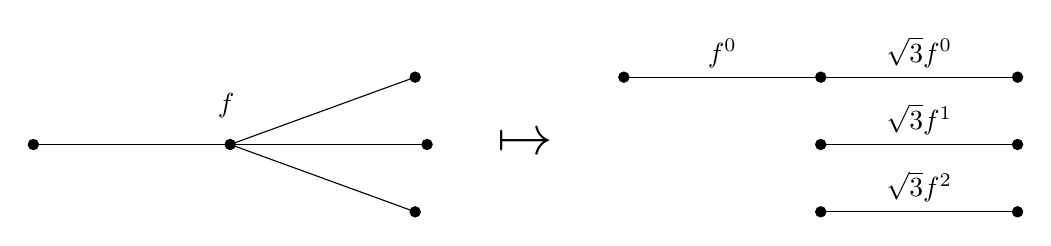
\begin{tikzpicture}[vertex/.style={draw,circle,minimum size=1.3mm,inner sep=0pt,outer sep=0pt,fill=black},scale=2.5]

    \draw (-1, 0) -- (0, 0);
    \node[vertex] at (-1, 0) {};
    \node[vertex] at (0, 0) {};

    \pgfmathsetmacro{\v}{20}

    \draw (0, 0) -- ({cos(\v)}, {sin(\v)});
    \node[vertex] at ({cos(\v)}, {sin(\v)}) {};

    \draw (0, 0) -- (1, 0);
    \node[vertex] at (1, 0) {};

    \draw (0, 0) -- ({cos(-\v)}, {sin(-\v)});
    \node[vertex] at ({cos(-\v)}, {sin(-\v)}) {};

    \draw (2, {sin(\v)}) -- (4, {sin(\v)});
    \node[vertex] at (2, {sin(\v)}) {};
    \node[vertex] at (3, {sin(\v)}) {};
    \node[vertex] at (4, {sin(\v)}) {};

    \node at (-0.02, 0.2) {$f$};

    \node[scale=2] at (1.5, 0) {$\mapsto$};

    \draw (3, 0) -- (4, 0);
    \node[vertex] at (3, 0) {};
    \node[vertex] at (4, 0) {};

    \draw (3, {sin(-\v)}) -- (4, {sin(-\v)});
    \node[vertex] at (3, {sin(-\v)}) {};
    \node[vertex] at (4, {sin(-\v)}) {};

    \node[above] at (2.5, {sin(\v)}) {$f^0$};
    \node[above] at (3.5, {sin(\v)}) {$\sqrt{3} f^0$};
    \node[above] at (3.5, 0) {$\sqrt{3} f^1$};
    \node[above] at (3.5, {sin(-\v)}) {$\sqrt{3} f^2$};

  \end{tikzpicture}
  \caption{The action of the transformation $U$ on $\Gamma_1$ with $m=3$.}
  \label{fig: U map}
\end{figure}

The matching conditions respect the symmetry of the graph, so scattering properties are invariant under the described rotations. Hence we need not distinguish between the edges in each generation when considering scattering properties, it is sufficient to study only $\widetilde{\Gamma}$ and take into account that each edge in generation $n$ represents all edges in generation $n$ in the original graph $\widetilde{\Gamma}$. We now set out to find the matching conditions on $\widetilde{\Gamma}$ that allow this transition from $\Gamma$ to $\widetilde{\Gamma}$.



\subsection{Matching conditions on the collapsed graph}

% We parametrize each edge $e_j$ from $0$ to $\abs{e_j}$, the length of the edge.
The original graph $\Gamma_1$ with inner vertex $v$ has standard matching conditions which can be written as follows
\[
  \begin{dcases}
    f_0(v) = f_j(v), \quad j = 1, 2, \ldots, m \\
    \partial f_0(v) + \sum_{j=1}^{m} \partial f_j(v) = 0.
  \end{dcases}
\]
In terms of the eigenfunctions $f^n$ of $R$ this can be written as
\begin{align*}
  n = 0: &
  \begin{dcases}
    f^0_0(v) = f^0_j(v), \quad j = 1, 2, \ldots, m  \\
    \Dop{x} f^0_0(v) = m \Dop{x} f^0_1(v)
  \end{dcases} \\
  n \ne 0: &
  \begin{dcases}
    0 = f^n_j(v), \quad j = 1, 2, \ldots, b \\
    \text{trivially satisfied: } \Dop{x} \underbrace{f^n_0(v)}_{=v} = \sum_{j=1}^m \Dop{x} f^n_j(v) = \Dop{x} f^n_1(v) \underbrace{\sum_{j=1}^{m} z^{n(j-1)}}_{=0}
  \end{dcases}
\end{align*}
We see that for the case $n \ne 0$ the continuity condition simply becomes the Dirichlet condition and for $n \ne 0$ the condition for the derivatives is trivially satisfied, as seen by using $f^n_j = z^{n(j-1)} f^n_1$. Thus we can write, for every $n$,
\begin{equation*}
  \Gamma_1:
  \begin{dcases}
    f^n_0(v) = f^n_j(v), \quad j = 1, 2, \ldots, m \\
    % \D{f^n_0}{x}(v) = m \D{f^n_1}{x}(v).
    \partial f^0_0(v) + m \partial f^0_1(v) = 0.
  \end{dcases}
\end{equation*}
Applying $U$ on the above conditions gives the matching conditions for the collapsed graph $\widetilde{\Gamma}_1$ gives the following result, where we have also used that the graph is self-similar, hence this analysis holds at every vertex of the graph.

\begin{proposition}[Collapsed snowflake matching conditions]
  Let $\Gamma$ be a quantum snowflake graph with branching number $m$ and standard matching conditions, let $\widetilde{\Gamma}$ be the corresponding collapsed graph (as described above). Then the two graphs $\Gamma$ and $\widetilde{\Gamma}$ have equal scattering properties if the matching conditions for $\widetilde{\Gamma}$ are chosen as
  \begin{equation}\label{eq: snowflake mc}
    % \widetilde{\Gamma}:
    \begin{dcases}
      f_0(v) = \frac{1}{\sqrt{m}} f_1(v) \\
      \partial f_0(v) + \sqrt{m} \partial f_1(v) = 0,
    \end{dcases}
  \end{equation}
  for every vertex $v$ in $\widetilde{\Gamma}$. Here $f_0$ denotes the restriction of $f$ to the edge attached to $v$ that is closest to the root of the graph, similarly $f_1$ denotes the restriction of $f$ to the edge attached to $v$ that is farthest away from the root of the graph.
\end{proposition}


We verify that $L$ still is self-adjoint on $\widetilde{\Gamma}_1$ under these new matching conditions. From equation \eqref{eq:self-adjoint_boundary_terms} we have that the following sum must vanish
\begin{align*}
  & \sum_{x \in v} \partial u(x)\overline{v}(x) - u(x)\partial\overline{v}(x) \\
  =& \Big(\partial u_0(v)\overline{v}_0(v) - u_0(v)\partial\overline{v}_0(v)\Big) + \Big(\partial u_0(v)\overline{v}_0(v) - u_0(v)\partial\overline{v}_0(v)\Big)
  % =& \Big(-u'(v)\overline{v}(v) + u(v)\overline{v}'(\ell_0)\Big) + \Big(u'(v)\overline{v}(v) - u(v)\overline{v}'(v)\Big)
\end{align*}
where $v$ is the inner vertex. Using the matching conditions we can write this as
\begin{align*}
  & \Big(-\sqrt{m} \partial u_1(v)\frac{1}{\sqrt{m}}\overline{v}_1(v) + \frac{1}{\sqrt{m}}u_1(v)\sqrt{m}\partial\overline{v}_1(v)\Big) + \Big(\partial u_1(v)\overline{v}_1(v) - u_1(v)\partial\overline{v}_1(v)\Big) \\
  =& -\Big(\partial u_1(v)\overline{v}_1(v) - u_1(v)\partial\overline{v}_1(v)\Big) + \Big(\partial u_1(v)\overline{v}_1(v) - u_1(v)\partial\overline{v}_1(v)\Big) = 0
\end{align*}

The following example illustrates how the collapsed graph compares to original graph for the case of a star graph.

\begin{example}[Collapsed snowflake of one generation]
  From section~\ref{sec: scattering from infinite star graph} we know that an infinite star graph $\Gamma$ of degree $d = m+1$ has transmission resp. reflection coefficient
  \begin{equation*}
    \begin{cases}
      T = 2/d \\
      R = 2/d - 1.
    \end{cases}
  \end{equation*}
  \begin{figure}[!h]
    \centering
    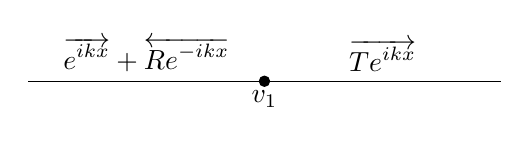
\begin{tikzpicture}[vertex/.style={draw,circle,minimum size=1.3mm,inner sep=0pt,outer sep=0pt,fill=black}, scale=3]
      \draw (-1,0) -- node[above] {$\overrightarrow{e^{ikx}} + \overleftarrow{Re^{-ikx}}$} (0,0) -- node[above] {$\overrightarrow{Te^{ikx}}$} (1,0);
      \node[vertex] at (0,0) {};
      \node[below] at (0,0) {$v_1$};
    \end{tikzpicture}
  \end{figure}
  In our new setting we collapse $\Gamma$ into $\widetilde{\Gamma}$ and apply the new matching conditions \eqref{eq: snowflake mc}
  \begin{align*}
    & \begin{dcases}
      1 + R = \frac{1}{\sqrt{m}} T \\
      1 - R = \sqrt{m} T
    \end{dcases}
    \implies
    \begin{dcases}
      T = \sqrt{m}\frac{2}{m+1} \\
      R = \frac{2}{m+1} - 1.
    \end{dcases}
  \end{align*}
  The factor $\sqrt{m}$ on the transmission coefficient can be seen as emerging from that all $m$ edges have been collapsed into one edge. The function on this edge can be seen as containing total information about the function an all edges in the same generation.
  We do indeed get the same scattering as for the ordinary star graph, the observed scattering is given by $\abs{R}^2$ and $\abs{T}^2$, the factor $m$ in $\abs{T}^2$ is due to the fact that there are $m$ edges into which the wave transmits.
\end{example}

By the self-similarity the snowflake graph, the matching conditions found in \ref{eq: snowflake mc} are valid for every vertex in the collapsed snowflake. We proceed to consider scattering in the collapsed graph.




\section{Scattering in the snowflake}\label{sec: scattering in the snowflake}

We attach a semi-infinite edge on the left end-point of the root edge $e_0$, which acts as our contact point to the graph. As we have seen in example~\ref{ex: remove vertex smc} we can disregard vertex $v_0$ since we have standard matching conditions there. The situation is indeed equivalent to giving edge $e_0$ infinite length. An incoming wave is sent along $e_0$ into the graph, we are interested in the resulting reflection $R$, see figure~\ref{fig: approaching the collapsed graph} and note that we are working on the collapsed graph $\widetilde{\Gamma}$.

\begin{figure}[!h]
  \centering
  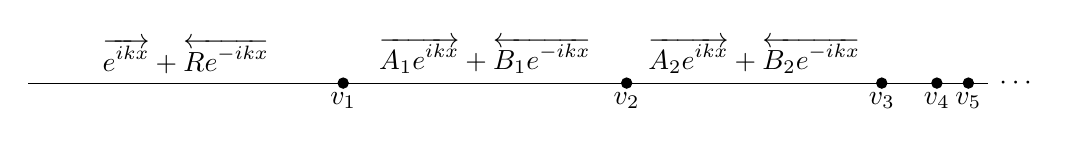
\begin{tikzpicture}[vertex/.style={draw,circle,minimum size=1.3mm,inner sep=0pt,outer sep=0pt,fill=black}, scale=1]
    \pgfmathsetmacro{\q}{0.9}
    \draw (-4,0) -- node[above] {$\overrightarrow{e^{ikx}} + \overleftarrow{Re^{-ikx}}$} (0,0) --
      node[above] {$\overrightarrow{A_1 e^{ikx}} + \overleftarrow{B_1 e^{-ikx}}$} ({4*\q^1},0) --
      node[above] {$\overrightarrow{A_2 e^{ikx}} + \overleftarrow{B_2 e^{-ikx}}$} ({4*\q^1+4*\q^2},0) --
      node[above] {} ({4*\q^1+4*\q^2+1.35},0);
    \node[vertex] at (0,0) {};
    \node[below] at (0,0) {$v_1$};
    \node[vertex] at ({4*\q^1},0) {};
    \node[below] at ({4*\q^1},0) {$v_2$};
    \node[vertex] at ({4*\q^1+4*\q^2},0) {};
    \node[below] at ({4*\q^1+4*\q^2},0) {$v_3$};
    \node[vertex] at ({4*\q^1+4*\q^2+0.7},0) {};
    \node[below] at ({4*\q^1+4*\q^2+0.7},0) {$v_4$};
    \node[vertex] at ({4*\q^1+4*\q^2+1.1},0) {};
    \node[below] at ({4*\q^1+4*\q^2+1.1},0) {$v_5$};
    % \node[vertex] at ({4*\q^1+4*\q^2+1.5},0) {};
    \node[] at ({4*\q^1+4*\q^2+1.7},0) {$\cdots$};
  \end{tikzpicture}
  \caption{Approaching the collapsed graph via a semi-infinite edge through the left end-point of the root edge $e_0$.}
  \label{fig: approaching the collapsed graph}
\end{figure}


On the entire collapsed graph, let $f_n$ be $f$ restricted to the (only) edge in generation $n$. We can then write the matching conditions at each vertex as
\begin{align*}
  &\begin{dcases}
    f_n(v_{n+1}) = \frac{1}{\sqrt{m}} f_{n+1}(v_{n+1}) \\
    \Dop{x} f_n(v_{n+1}) = \sqrt{m} \Dop{x} f_{n+1}(v_{n+1})
  \end{dcases} \\
  \iff &\begin{dcases}
    A_n e^{ik\beta^n} + B_n e^{ik\beta^n} = \frac{1}{\sqrt{m}} \big( A_{n+1} + B_{n+1} \big) \\
    A_n e^{ik\beta^n} - B_n e^{ik\beta^n} = \sqrt{m} \big( A_{n+1} - B_{n+1} \big).
  \end{dcases}
\end{align*}

To find the resulting reflection $R$ we will first consider reflection and transmission from one single vertex.




\subsection{Scattering coefficients at vertices in the collapsed graph}\label{sec: scattering at vertex}

We seek to calculate the reflection and transmission coefficients from left and right through any vertex in the snowflake. Because of the self-similarity of the graph, it suffices to consider just one vertex, the situation will be the same for all other vertices. To calculate this, we need to disregard reflections from other vertices in the graph. Hence, we consider an infinite snowflake of one generation, i.e.\ an infinite line graph with one vertex at which we have snowflake matching conditions, c.f.\ figure~\ref{fig: reflection transmission coefficients}.

\begin{figure}[!h]
  \centering
  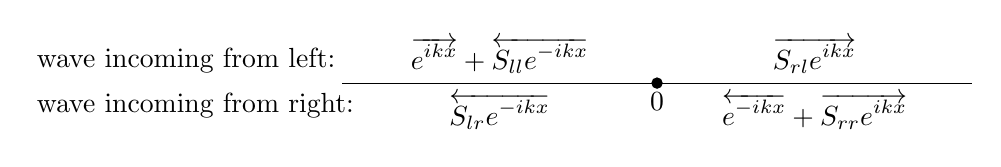
\begin{tikzpicture}[vertex/.style={draw,circle,minimum size=1.3mm,inner sep=0pt,outer sep=0pt,fill=black}, scale=1]
    \draw (-4,0) -- (0,0) -- (4,0);
    \node[vertex] at (0,0) {};
    \node[below] at (0,0) {$0$};

    \node[above] at (-2,0) {$\overrightarrow{e^{ikx}} + \overleftarrow{S_{ll} e^{-ikx}}$};
    \node[above] at (2,0)  {$\overrightarrow{S_{rl} e^{ikx}}$};

    \node[below] at (-2,0) {$\overleftarrow{S_{lr} e^{-ikx}}$};
    \node[below] at (2,0)  {$\overleftarrow{e^{-ikx}} + \overrightarrow{S_{rr} e^{ikx}}$};

    \node[above right] at (-8,0) {wave incoming from left:};
    \node[below right] at (-8,0) {wave incoming from right:};
  \end{tikzpicture}
  \caption{Incoming wave from left resp.\ right. in an infinite line graph with snowflake matching conditions.}
  \label{fig: reflection transmission coefficients}
\end{figure}

For a wave incoming from the left, $S_{ll}$ is the amplitude of the reflected wave and $S_{rl}$ of the transmitted wave. Similarly, for a wave incoming from the right, $S_{rr}$ is the amplitude of the reflected wave and $S_{lr}$ of the transmitted wave. Compare the notation to the $S$-matrix in section~\ref{sec: scattering phenomena}. From the snowflake matching conditions \eqref{eq: snowflake mc} we have
\begin{align*}
  \text{wave incoming from left:} & \begin{dcases}
    1 + S_{ll} = \frac{1}{\sqrt{m}} S_{rl} \\
    1 - S_{ll} = \sqrt{m} S_{rl}
  \end{dcases}
  && \implies \begin{dcases}
    S_{ll} = \frac{1-m}{1+m} \\
    S_{rl} = \frac{2\sqrt{m}}{1+m}
  \end{dcases}
  \\
  \text{wave incoming from right:} & \begin{dcases}
    S_{lr} = \frac{1}{\sqrt{m}} \big( 1 + S_{rr} \big) \\
    -S_{lr} = \sqrt{m} \big( - 1 + S_{rr} \big)
  \end{dcases}
  && \implies \begin{dcases}
    S_{rr} = -\frac{1-m}{1+m} \\
    S_{lr} = \frac{2\sqrt{m}}{m+1}.
  \end{dcases}
\end{align*}
Evidently $S_{rr} = - S_{ll}$ and $S_{rl} = S_{lr}$, but in what follows we will often distinguish between left and right transmission and reflection to emphasize which path the wave has taken through the graph.




\subsection{Scattering from a snowflake of 2 generations}\label{sec: scattering 2 gen snowflake}

We now set out study how waves get transmitted and reflected in finite edges in a snowflake. We begin by considering a collapsed snowflake with two generations where the second generation is assigned infinite length through which the wave is allowed to escape (cf.\ remark~\ref{rem: semi-infinite edges for scattering}). Through this simplified snowflake we study transmission and reflection due to the two vertices $v_1$ and $v_2$, later on we will successively add back all vertices and edges to get back the snowflake graph.
% We parametrize the resulting line graph from $-\infty$ to $\infty$ with $x = x_i$ at $v_i$.

\begin{figure}[!h]
  \centering
  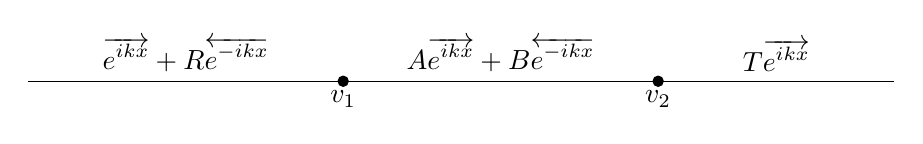
\begin{tikzpicture}[vertex/.style={draw,circle,minimum size=1.3mm,inner sep=0pt,outer sep=0pt,fill=black}, scale=1]
    \draw (-4,0) -- (0,0) -- (4,0) -- (7,0);

    \node[vertex] at (0,0) {};
    \node[below] at (0,0) {$v_1$};

    \node[vertex] at (4,0) {};
    \node[below] at (4,0) {$v_2$};

    \node[above] at (-2,0) {$\overrightarrow{e^{ikx}} + R \overleftarrow{e^{-ikx}}$};
    \node[above] at (2,0) {$A \overrightarrow{e^{ikx}} + B \overleftarrow{e^{-ikx}}$};
    \node[above] at (5.5,0) {$T \overrightarrow{e^{ikx}}$};
  \end{tikzpicture}
  \caption{A finite snowflake with 2 generations}
\end{figure}

As the incoming wave reaches vertex $v_1$, part of the wave gets reflected and part of it gets transmitted. All waves on edge $e_1$ will have been transmitted through $v_1$ once and reflected at $v_2$ to the left followed by reflection at $v_1$ to the right, etc. Hence the total wave on edge $e_1$ is
\begin{equation}\label{eq: bouncing waves}
  \begin{aligned}
    & S_{rl} \overrightarrow{e^{ik(x-v_1)}} + \\
    & S_{rl} e^{ik(v_2-v_1)} S_{ll} \overleftarrow{e^{-ik(x-v_2)}} + \\
    & S_{rl} e^{ik(v_2-v_1)} S_{ll} e^{-ik(v_1-v_2)} S_{rr} \overrightarrow{e^{ik(x-v_1)}} + \\
    & S_{rl} e^{ik(v_2-v_1)} S_{ll} e^{-ik(v_1-v_2)} S_{rr} e^{ik(v_2-v_1)} S_{ll} \overleftarrow{e^{-ik(x-v_2)}} + \\
    & S_{rl} e^{ik(v_2-v_1)} S_{ll} e^{-ik(v_1-v_2)} S_{rr} e^{ik(v_2-v_1)} S_{ll} e^{-ik(v_1-v_2)} S_{rr} \overrightarrow{e^{ik(x-v_2)}} + \ldots
    % & S_{rl} e^{ik(v_2-v_1)} S_{ll} e^{-ik(v_1-v_2)} S_{rr} e^{ik(v_2-v_1)} S_{ll} e^{-ik(v_1-v_2)} S_{rr} e^{ik(v_2-v_1)} S_{ll} \overleftarrow{e^{-ik(x-v_2)}} + \ldots
    % & \vdots
  \end{aligned}
\end{equation}
Letting $\ell_1 = v_2-v_1 = \ell_0\beta$ and separating the left traveling waves from the right traveling waves gives
\begin{align*}
  A \overrightarrow{e^{ik(x-v_1)}} &= S_{rl} e^{ik(x-v_1)} \left(1 + e^{2ik\ell_1} S_{ll} S_{rr} + \left(e^{2ik\ell_1} S_{ll} S_{rr}\right)^2 + \ldots \right) \overrightarrow{e^{ik(x-v_1)}} \\
  &= \frac{S_{rl}}{1-e^{2ik\ell_1}S_{ll}S_{rr}} \overrightarrow{e^{ik(x-v_1)}} \\
  B \overleftarrow{e^{-ik(x-v_1)}} &= S_{rl} S_{ll} e^{ik\ell_1} e^{-ik(x-v_2)} \left(1 + e^{2ik\ell_1} S_{rr} S_{ll} +  \left(e^{2ik\ell_1} S_{rr} S_{ll}\right)^2 + \ldots \right) \overleftarrow{e^{-ik(x-v_2)}} \\
  &= \frac{e^{ik\ell_1} S_{rl} S_{ll}}{1 - e^{2ik\ell_1} S_{ll} S_{rr}} \overleftarrow{e^{-ik(x-v_2)}}.
\end{align*}
These geometric series satisfy $|e^{2ik\ell_1}S_{ll}S_{rr}| < 1$ since it always holds that $\abs{S_{ll}}^2 + \abs{S_{rl}}^2 = 1$ and $\abs{S_{rr}}^2 + \abs{S_{lr}}^2 = 1$, we also have $\abs{S_{ij}} > 0$, thus we conclude $\abs{S_{ij}} < 1$, where $i,j = l,r$.

The total escaping wave is given by waves being transmitted through $v_1$ followed by any number of reflections back and forth on edge $e_1$, between vertices $v_1$ and $v_2$, and finally transmitted through $v_2$. That is, using the results from the above calculations,
\begin{gather}\label{eq: transmission 2 generation snowflake}
  \begin{aligned}
    T \overrightarrow{e^{ik(x-v_2)}} &= S_{rl} e^{ik\ell_1} \left( 1 + e^{2ik\ell_1} S_{ll} S_{rr} + \left(e^{2ik\ell_1} S_{ll} S_{rr}\right)^2 + \ldots \right) S_{rl} \overrightarrow{e^{ik(x-v_2)}} \\
    &= \frac{e^{ik\ell_1} S_{rl}^2}{1 - e^{2ik\ell_1} S_{ll} S_{rr}} \overrightarrow{e^{ik(x-v_2)}}.
  \end{aligned}
\end{gather}
Note that this is precisely $A e^{ikv_2} S_{rl} e^{ik(x-v_2)}$, where $A e^{ikx}$ has already been calculated. Using this observation we can directly write down the expression for the total wave being reflected back from the graph by realizing that such a wave is either the wave being directly reflected at $v_1$ or any of the left traveling waves on $e_1$ being transmitted through $v_1$,
\begin{gather}\label{eq: reflection 2 generation snowflake}
  \begin{aligned}
    R \overleftarrow{e^{-ik(x-v_1)}} &= S_{ll} \overleftarrow{e^{-ik(x-v_1)}} + B e^{-ikv_1} S_{lr} \overleftarrow{e^{-ik(x-v_1)}} \\
    &= \left( S_{ll} + \frac{e^{2ik\ell_1} S_{rl} S_{ll} S_{lr}}{1 - e^{2ik\ell_1} S_{ll} S_{rr}} \right) \overleftarrow{e^{-ik(x-v_1)}}.
  \end{aligned}
\end{gather}

Substituting in the values of the scattering coefficients gives
\begin{equation}\label{eq: scattering coefficients 2 generation snowflake}
  \begin{aligned}
    R  &= -\frac{(m^2-1)(1 + e^{2ik\ell_1})}{(m+1)^2 + e^{2ik\ell_1} (m-1)^2} \\
    % -\frac{\left(m^2-1\right) \cos (k \ell_1)}{\left(m^2+1\right) \cos (k \ell_1) - 2 i m \sin (k \ell_1)}.
    T &=  \frac{4m e^{ik\ell_1}}{(m+1)^2+e^{2ik\ell_1}(m-1)^2}
  \end{aligned}
\end{equation}
and
\[
  \abs{R}^2 = \frac{(m^2-1)^2 \cos^2(kl)}{(m^2+1)^2 \cos^2(kl) + 4m^2\sin^2(kl)}.
\]
In section~\ref{sec: radial graphs} the equivalent non-collapsed graph with standard matching conditions was studied. If we let $b_1 = b_2 = m$, i.e.\ set all branching numbers equal to $m$, in the equation \eqref{eq: 2gen R} for $R$, we recover the above expression. One benefit of the method developed here is that it gives more information about how the wave propagates and reflects in the graph, and it is easier to generalize to $n$ generations. To do this we will further reduce the complexity of the graph by merging vertices.



\section{Merging vertices}

Ideally we would like to continue the above procedure for additional generations of the graph. Repeating the same procedure without modification is however not possible since, unlike the case for only just one finite generation, there will be an infinite number of different types of possible paths for the wave to take. To see this we introduce a labeling for each possible path that the wave can take.

To each path we assign a sequence of integers, each integer corresponding to the generation that the wave goes through. For example, in the case of 2 generations, every path first propagates on $e_0$, giving 0 as the first number of the sequence. This is followed by any number of reflections on $e_1$, hence the next numbers in the sequence are any number of 1's. This is finally followed by either transitioning to $e_0$ or $e_{11}$. Hence the possible sequences are
\[ 0\underbrace{111\ldots111}_{\text{even}}0 \quad \text{ and } \quad 0\underbrace{111\ldots111}_{\text{odd}}2. \]
The first class of sequences corresponds to waves being reflected, contributing to $R$, and the second class similarly corresponds to transmissions, contributing to $T$, compare with expressions \eqref{eq: bouncing waves}. With some elementary computations one shows that $\abs{R}^2 + \abs{T}^2 = 1$, implying that no waves `get stuck' on the middle edge $e_1$. That is, even though the sequence need not necessarily terminate, it may look as $0111\ldots$, but the corresponding amplitude for this sequence vanishes.

For three generations there are an infinite number of possible types of sequences, for example we have the sequences
\[ 0122112211\ldots, \quad 01222211222211\ldots, \quad 011122111122\ldots, \]
etc. In contrast to the case of 2 generations we had only $2$ types of such strings. This makes it very difficult to proceed as we did for two generations when we wrote down \eqref{eq: bouncing waves}. Note however, just as for the case of 2 generations, all contributing waves correspond to sequences ending with 0 or 3, corresponding to reflection and transmission respectively. We will now develop a method study reflection when additional edges are added.

Analogously to how we collapsed all edges in each generation into one edge using the rotational symmetry of the graph to reduce the complexity, we will now combine two vertices into one, to further reduce the complexity of the graph. As we saw for the case of 2 generations, $\abs{R}^2 + \abs{T}^2 = 1$, allows us to regard the subgraph consisting of one middle edge and its two vertices, as one larger vertex, see figure~\ref{fig: combine vertices}.

\begin{figure}[!h]
  \centering
  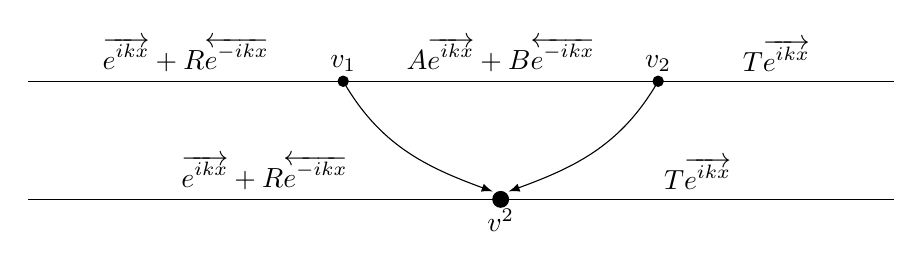
\begin{tikzpicture}[vertex/.style={draw,circle,minimum size=1.3mm,inner sep=0pt,outer sep=0pt,fill=black}, scale=1]
    \draw (-4,0) -- (7,0);

    \node[vertex] at (0,0) {};
    \node[above] at (0,0) {$v_1$};

    \node[vertex] at (4,0) {};
    \node[above] at (4,0) {$v_2$};

    \node[above] at (-2,0) {$\overrightarrow{e^{ikx}} + R \overleftarrow{e^{-ikx}}$};
    \node[above] at (2,0) {$A \overrightarrow{e^{ikx}} + B \overleftarrow{e^{-ikx}}$};
    \node[above] at (5.5,0) {$T \overrightarrow{e^{ikx}}$};

    \pgfmathsetmacro{\y}{-1.5}
    \draw (-4,\y) -- (7,\y);

    \node[vertex,style={minimum size=2mm}] at (2,\y) {};
    \node[below] at (2,\y) {$v^2$};

    \draw[-latex] (0,0) to[out=300,in=160,looseness=1] (1.9,{\y+0.1});
    \draw[-latex] (4,0) to[out=240,in=20 ,looseness=1] (2.1,{\y+0.1});

    \node[above] at (-1,\y) {$\overrightarrow{e^{ikx}} + R \overleftarrow{e^{-ikx}}$};
    \node[above] at (4.5,\y) {$T \overrightarrow{e^{ikx}}$};
  \end{tikzpicture}
  \caption{Combining two vertices into one.}
  \label{fig: combine vertices}
\end{figure}

% \begin{figure}[!h]
%   \centering
%   \begin{tikzpicture}[vertex/.style={draw,circle,minimum size=1.3mm,inner sep=0pt,outer sep=0pt,fill=black}, scale=1]
%     \draw (-3,0) -- (9,0);

%     \node[vertex] at (0,0) {};
%     \node[below] at (0,0) {$x_1$};

%     \node[vertex] at (3.5,0) {};
%     \node[below] at (3.5,0) {$x_2$};

%     \node[vertex] at (7,0) {};
%     \node[below] at (7,0) {$x_2$};

%     \node[above] at (-1.5,0) {$\overrightarrow{e^{ikx}} + R \overleftarrow{e^{-ikx}}$};
%     \node[above] at (1.75,0) {$A \overrightarrow{e^{ikx}} + B \overleftarrow{e^{-ikx}}$};
%     \node[above] at (5.25,0) {$A_2 \overrightarrow{e^{ikx}} + B_2 \overleftarrow{e^{-ikx}}$};
%     \node[above] at (8,0) {$T \overrightarrow{e^{ikx}}$};
%   \end{tikzpicture}
%   \caption{A finite snowflake with 3 generations}
% \end{figure}

The graph we get after merging vertex $v_1$ with $v_2$ into one vertex, denoted $v^2$ will have edge $e_1$ removed and hence the total length reduced by $\ell_0\beta$. This causes no problem since we are only interested in scattering properties of the graph. We have already concluded that using non-continuous parametrization for the edges of the snowflake will, at worst, introduce a phase shift for the probability amplitude, hence $\abs{R}^2$ is unaffected. Indeed, we have used this repeatedly when working with different parametrizations. To preserve the scattering properties of the graph it suffices to ensure that the combined scattering coefficients for the vertices located at $v_1$ and $v_2$ are equal to those of the combined vertex at $v^2$ in the reduced graph, c.f.\ figure~\ref{fig: combine vertices}.

Denote the scattering coefficients for the merged vertex by $S_{2,ij}$ for $i,j=l,r$, to indicate that the scattering coefficient represents scattering from 2 ordinary vertices. In equations \eqref{eq: transmission 2 generation snowflake} and \eqref{eq: reflection 2 generation snowflake} we saw that
\begin{align*}
  S_{2,ll} &= S_{ll} + \frac{e^{2ik\ell_1} S_{rl} S_{ll} S_{lr}}{1 - e^{2ik\ell_1} S_{ll} S_{rr}} \\
  S_{2,rl} &= \frac{e^{ik\ell_1} S_{rl}^2}{1 - e^{2ik\ell_1} S_{ll} S_{rr}}.
\end{align*}
To proceed and determine $S_{3,ll}$ etc.\ we must also determine $S_{2,rr}$ and $S_{2,lr}$, however this is easy when we have the above expressions. Indeed, for the case of an incoming wave from the right, the internal scattering is precisely as for the case of an incoming wave from the left, with the modification that everything is mirror reflected. That is, every occurrence of $S_{ij}$ is replaced by $S_{ji}$, for $j,i=l,r$. Hence we have
\begin{align*}
  S_{2,rr} &= S_{rr} + \frac{e^{2ik\ell_1} S_{lr} S_{rr} S_{rl}}{1 - e^{2ik\ell_1} S_{rr} S_{ll}} \\
  S_{2,lr} &= \frac{e^{ik\ell_1} S_{lr}^2}{1 - e^{2ik\ell_1} S_{rr} S_{ll}}.
\end{align*}
Recall $S_{ll} = -S_{rr}$ and $S_{lr} = S_{rl}$, hence we see that this relation is preserved for the collapsed merged coefficients, that is $S_{2,ll} = -S_{2,rr}$ and $S_{2,lr} = S_{2,rl}$.



\section{Recursive expression for reflection from $n$ generations}

We now proceed by merging additional edges. Let $v^n$ denote the vertex created by merging vertices $v_1, v_2, \ldots, v_n$, let $S_{ij,n}$ for $i,j=l,r$ denote the scattering coefficient for vertex $v^n$, and let $\ell_n = d(v^{n-1}, v_n) = \ell_0\beta^n$ denote the distance between vertex $v^{n-1}$ and $v_n$.

\begin{figure}[!h]
  \centering
  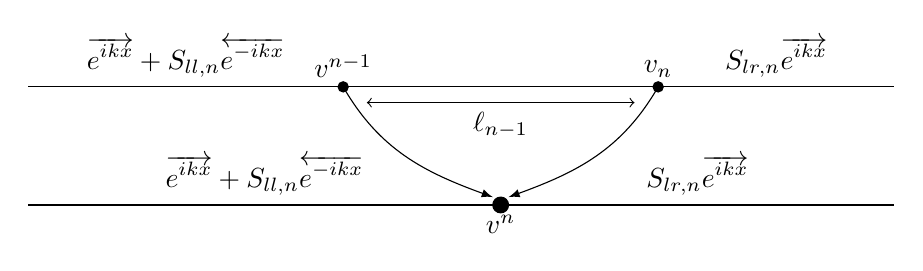
\begin{tikzpicture}[vertex/.style={draw,circle,minimum size=1.3mm,inner sep=0pt,outer sep=0pt,fill=black}, scale=1]
    \draw (-4,0) -- (7,0);

    \node[vertex] at (0,0) {};
    \node[above] at (0,0) {$v^{n-1}$};

    \node[vertex] at (4,0) {};
    \node[above] at (4,0) {$v_n$};

    \node[above] at (-2,0) {$\overrightarrow{e^{ikx}} + S_{ll,n} \overleftarrow{e^{-ikx}}$};
    \node[above] at (5.5,0) {$S_{lr,n} \overrightarrow{e^{ikx}}$};

    \pgfmathsetmacro{\y}{-1.5}
    \draw (-4,\y) -- (7,\y);

    \node[vertex,style={minimum size=2mm}] at (2,\y) {};
    \node[below] at (2,\y) {$v^n$};

    \draw[<->] ({0+0.3},-0.2) to ({4-0.3},-0.2);
    \node[below] at (2,-0.2) {$\ell_{n-1}$};

    \draw[-latex] (0,0) to[out=300,in=160,looseness=1] (1.9,{\y+0.1});
    \draw[-latex] (4,0) to[out=240,in=20 ,looseness=1] (2.1,{\y+0.1});

    \node[above] at (-1,\y) {$\overrightarrow{e^{ikx}} + S_{ll,n} \overleftarrow{e^{-ikx}}$};
    \node[above] at (4.5,\y) {$S_{lr,n} \overrightarrow{e^{ikx}}$};
  \end{tikzpicture}
  \caption{Combining a merged vertex with an ordinary vertex.}
  \label{fig: combine vertices 2}
\end{figure}

Every step in the procedure of merging vertices has the same structure, the $(n-1)$:th step merges vertex $v^{n-1}$ with $v_n$ into $v^n$, cf.\ figure~\ref{fig: combine vertices 2}. Hence we can directly write down a recursive expression for the resulting reflection $S_{ll,n}$ of a snowflake graph with $n$ generations as follows.

\begin{proposition}
  Let $\Gamma$ be a quantum snowflake graph with $n+1$ generations, branching number $m$ and edge length $\ell_j$ in generation $j$. Then the total reflection $R_{n+1}(k) = S_{ll,n+1}(k)$ is given by the recursion formula
  \begin{equation}\label{eq: recursion}
    \begin{aligned}
      \text{recursion: } & \left\lbrace\!\!
      \begin{aligned}
        S_{ll,n+1} &= S_{ll,n} + \frac{e^{2ik\ell_n} S_{rl,n} S_{ll,1} S_{lr,n}}{1 - e^{2ik\ell_n} S_{rr,n} S_{ll,1}} \\
        S_{rl,n+1} &= \frac{e^{ik\ell_n} S_{rl,n} S_{rl,1}}{1 - e^{2ik\ell_n} S_{ll,1} S_{rr,n}} \\
        % S_{rr,n+1} &= -S_{ll,n} \\
        S_{rr,n+1} &= S_{rr,1} + \frac{e^{2ik\ell_n} S_{lr,1} S_{rr,n} S_{rl,1}}{1 - e^{2ik\ell_n} S_{ll,1} S_{rr,n}} \\
        % S_{lr,n+1} &= S_{rl,n}
        S_{lr,n+1} &= \frac{e^{ik\ell_n} S_{lr,1}S_{lr,n}}{1 - e^{2ik\ell_n} S_{rr,n} S_{ll,1}} \\
      \end{aligned}\right. \\
      \text{base case: } & \left\lbrace\!\!
      \begin{aligned}
        S_{ll,1} &= \frac{1-m}{1+m} \\
        S_{rl,1} &= \frac{2\sqrt{m}}{1+m} \\
        S_{rr,1} &= -S_{ll,1} \\
        S_{lr,1} &= S_{rl,1}
      \end{aligned}\right.
    \end{aligned}
  \end{equation}
\end{proposition}

Note that for $S_{rr,n+1}$ and $S_{lr,n+1}$ the scattering process is reversed in comparison to $S_{ll,n+1}$ and $S_{rl,n+1}$ respectively. That is, each occurrence of $S_{ij,n}$ is replaced by $S_{ji,1}$ and vice versa, where $i,j=r,l$.

% Simplify this using $S_{ll,n} = -S_{rr,n}$ and $S_{rl,n} = S_{,lr}$, and furthermore writing $R_n = S_{ll,n}$ and $T_n = S_{rl,n}$, gives
% \begin{align}
%   \begin{split}\label{eq: recursive Rn}
%     R_{n+1} &= S_{ll,n} + \frac{e^{2ik\ell_0\beta^n} S_{rl,n} S_{ll,n} S_{lr,n}}{1 - e^{2ik\ell_0\beta^n} S_{ll,n} S_{rr,n}} \\
%     &= R_n \g{ 1 + \frac{e^{2ik\ell_0\beta^n} T_n^2}{1 + e^{2ik\ell_0\beta^n} R_n^2} } \\
%     &= R_n \frac{1 + e^{2ik\ell_0\beta^n} \g{ R_n^2 + T_n^2 }}{1 + e^{2ik\ell_0\beta^n} R_n^2},
%   \end{split} \\
%   \begin{split}
%     T_{n+1} &= \frac{e^{ik\ell_0\beta^n} S_{rl,n}^2}{1 - e^{2ik\ell_0\beta^n} S_{ll,n} S_{rr,n}} \\
%     &= \frac{e^{ik\ell_0\beta^n} T_n^2}{1 + e^{2ik\ell_0\beta^n} R_n^2}.
%   \end{split}
% \end{align}
% Unfortunately $R_n^2 + T_n^2 \ne 1$ for $n>1$ since $R_n$ and $T_n$ are complex in general, this would have allowed us to make a major simplification to the expression for $R_{n+1}$.

The reflection from a complete snowflake is now indeed given by the limit
\[
  R(k,m,\beta) = \lim_{n\to\infty} S_{ll,n}(k,m,\beta).
\]
However, it is very difficult to say much about this in general, based on the recursion expression. Indeed, the reflection admits very complex behavior already for 5 generations. In figure~\ref{fig: snowflake reflection graphs} the reflection from snowflakes with varying parameters and up to 8 generations is shown. We have already seen that the reflection coefficient $R_2(k)$ is periodic in $k$ for $n=2$ generations, this is however not the case in general. Ineed, for $n=3$ generations we get the reflection coefficient
\begin{multline*}
  S_{3,ll} = -\frac{(m-1) \left((m-1)^2 e^{2 i \beta^3 k \ell_0}+(m+1)^2 e^{2 i \beta^2 k \ell_0}+(m+1)^2 e^{2 i \beta^2 (\beta+1) k
     \ell_0}+(m+1)^2\right)}{(m+1) \left((m-1)^2 e^{2 i \beta^3 k \ell_0}+(m-1)^2 e^{2 i \beta^2 k \ell_0}+(m-1)^2 e^{2 i \beta^2
     (\beta+1) k \ell_0}+(m+1)^2\right)}
 %  S_{3,ll} = -\frac{(m-1) \left((m-1)^2 e^{2 i \beta^2 \ell_0 k}+(m+1)^2 e^{2 i \beta \ell_0 k}+(m+1)^2 e^{2 i \beta (\beta+1) k
 % \ell_0  }+(m+1)^2\right)}{(m+1) \left((m-1)^2 e^{2 i \beta^2 \ell_0 k}+(m-1)^2 e^{2 i \beta \ell_0 k}+(m-1)^2 e^{2 i \beta (\beta+1) k
 % \ell_0  }+(m+1)^2\right)}
\end{multline*}
which is periodic if and only if there exist values for $k$ such that all phases equal a multiple of $2\pi$. This is a strong condition that is generally not satisfied. In particular we must have $2\beta^2 k\ell_0 = 2\pi s_1$ and $2\beta^3 k\ell_0 = 2\pi s_2$ for integers $s_1$ and $s_2$. This implies $\beta = s_1/s_2$, which is satisfied only if $\beta$ is a rational number. Next, also the phase $2\beta^2(\beta+1)k\ell_0$ must equal $2\pi s_3$ for some integer $s_3$, further strengthening the condition for the reflection to be periodic. This indicates that a general snowflake with arbitrary $\beta$ and high number $n$ of generations is not periodic.

As indicated by the plots, for fixed $k$ the reflection increases if $m$ increases.
\begin{lemma}
  Let $\Gamma$ and $\Gamma'$ be two quantum snowflake graphs with branching number $m$ and $m'$ respectively. If $m > m'$ then
  \[
    \abs{R_m(k)}^2 \ge \abs{R_{m'}(k)}^2
  \]
  with equality only for $k$ satisfying $\abs{R_m(k)}^2 = 0$ or $\abs{R_m(k)}^2 = 1$.
\end{lemma}
\noindent Indeed, this is clear from the recursive expression \eqref{eq: recursion}: the branching number $m$ appears only in the base case, which increasing $m$ increases $\abs{S_{ll,1}}^2$, this in turn causes $\abs{S_{ll,2}}^2$ to increase etc.

Thus the case $m=2$ is generally the most interesting branching number. Recall that for $m=1$ there is no reflection at all, we get a simple line graph with standard matching conditions.
% The plots also indicate that in general there are intervals of energies for which total reflection is achieved, the converse does not seem to hold, although there are energy regions where most of the wave gets absorbed in the graph.

To give a satisfactory answer to how the reflection from the snowflake graph behaves for arbitrary values of the parameter $\beta$ as $n\to\infty$ would require further analysis. The seemingly chaotic behavior makes this very difficult. However, the case $\beta = 1$, giving a periodic graph, is fully analyzed in the subsequent section.
% For the other values of $\beta$, the above discussion of periodicity indicates that the case $\beta = 1/2$ admits the shortest period, this will however not be studied in this text.


\begin{figure}[!h]
  \begin{subfigure}[t]{\textwidth}
    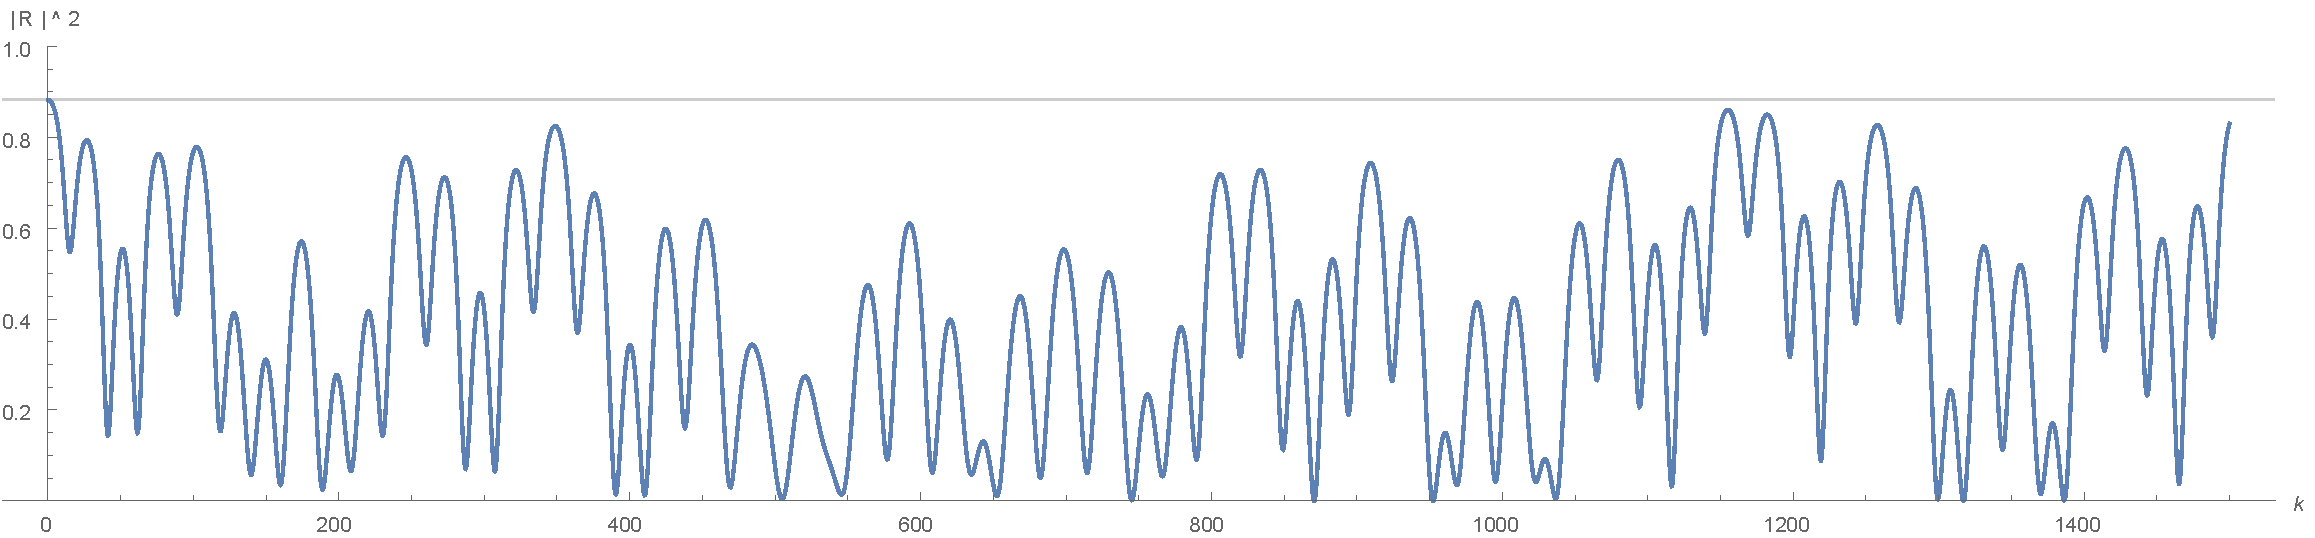
\includegraphics[width=1\textwidth]{img/reflection_n=5_m=2_l=1_b=03_kmax=1500}
    \caption{$n=5, m=2, \ell_0=1, \beta=0.3$}
  \end{subfigure}
  % \begin{subfigure}[t]{\textwidth}
  %   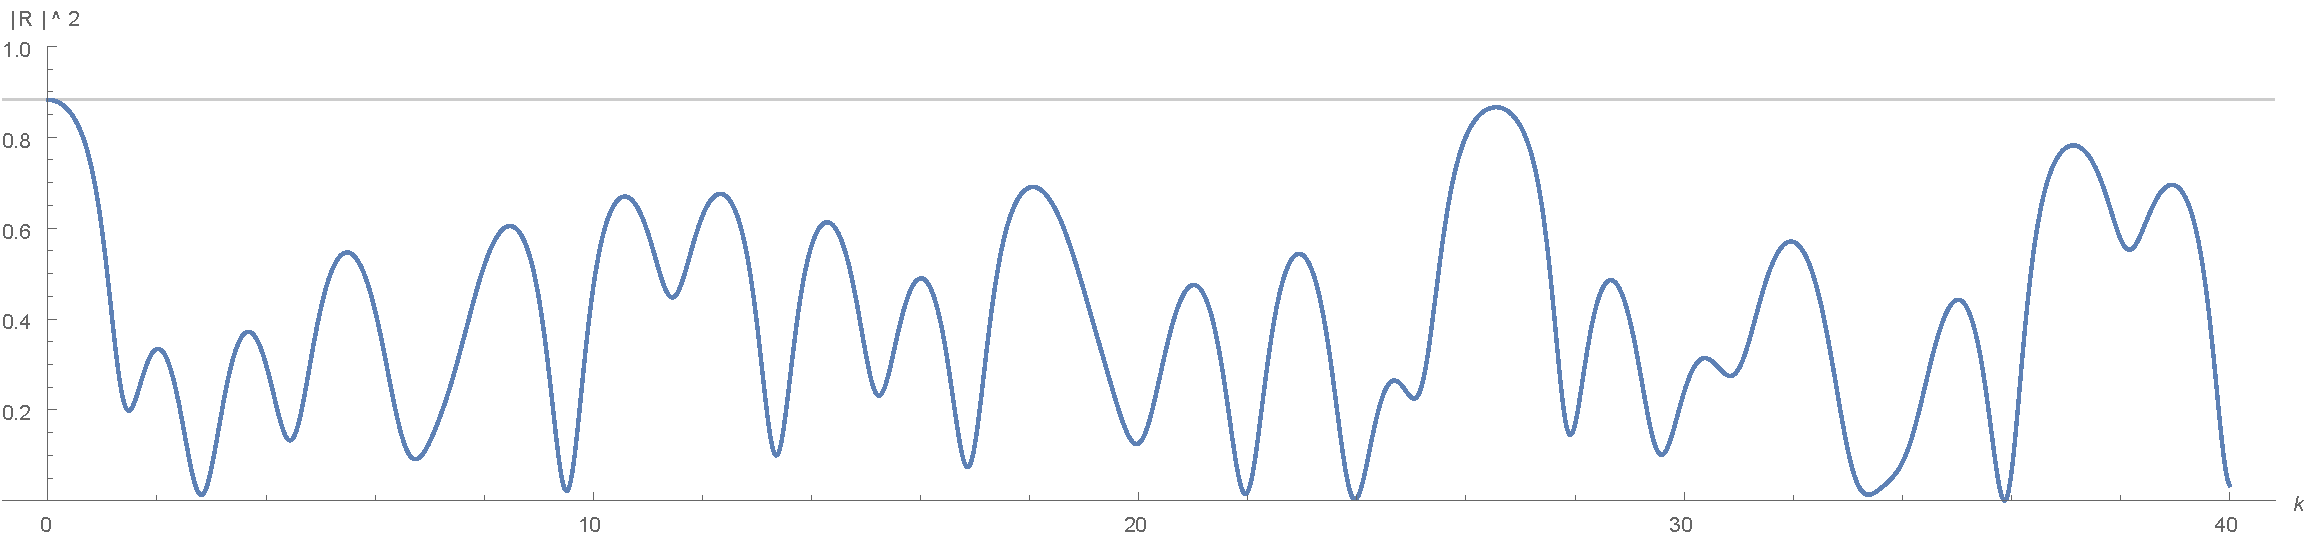
\includegraphics[width=1\textwidth]{img/reflection_n=5_m=2_l=1_b=07_kmax=40}
  %   \caption{$n=5, m=2, \ell_0=1, \beta=0.7$}
  % \end{subfigure}
  \begin{subfigure}[t]{\textwidth}
    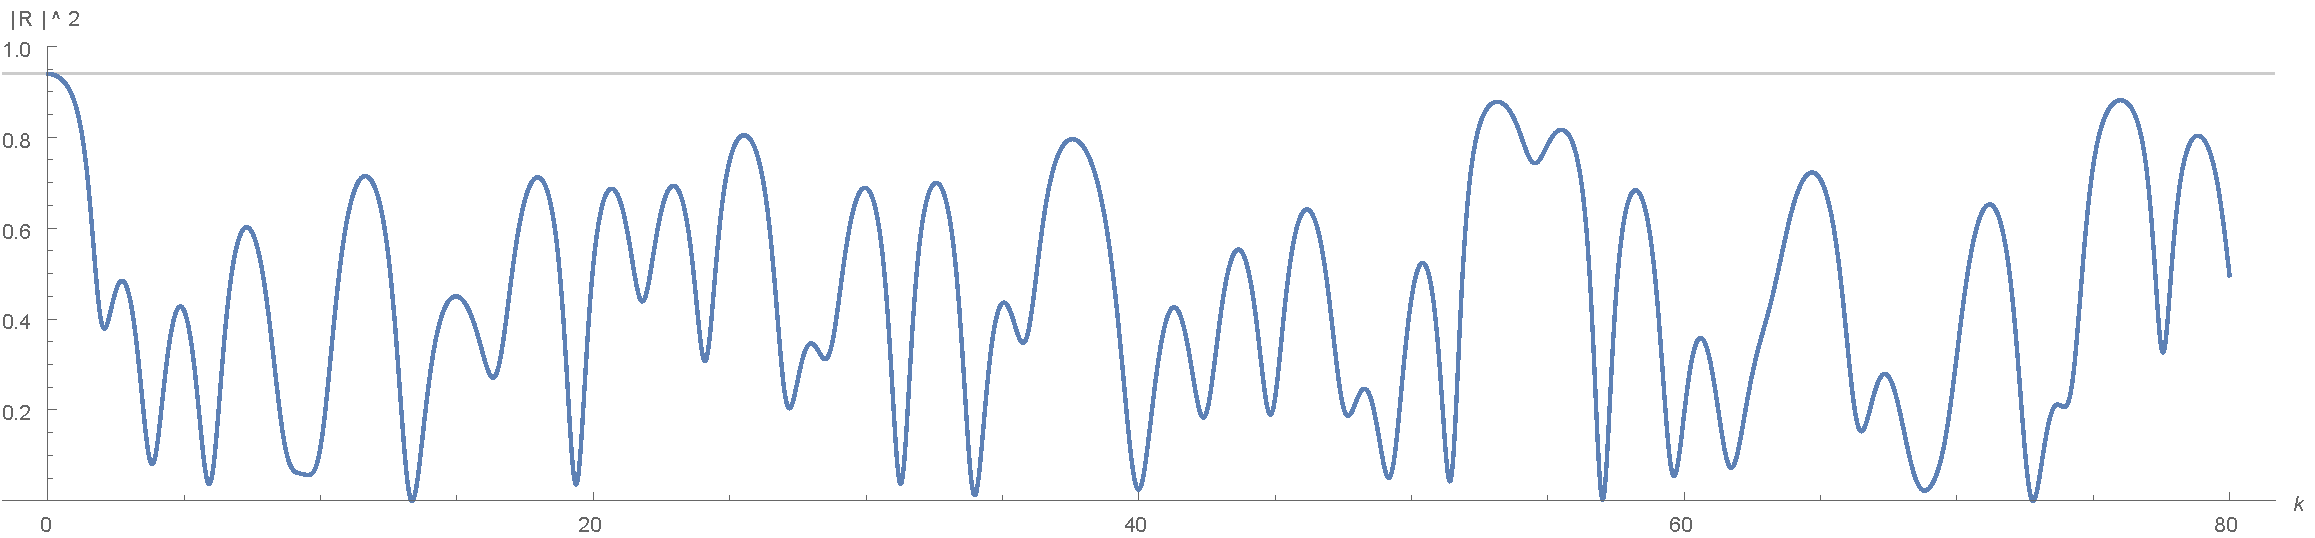
\includegraphics[width=1\textwidth]{img/reflection_n=6_m=2_l=1_b=07_kmax=80}
    \caption{$n=6, m=2, \ell_0=1, \beta=0.7$}
  \end{subfigure}
  \begin{subfigure}[t]{\textwidth}
    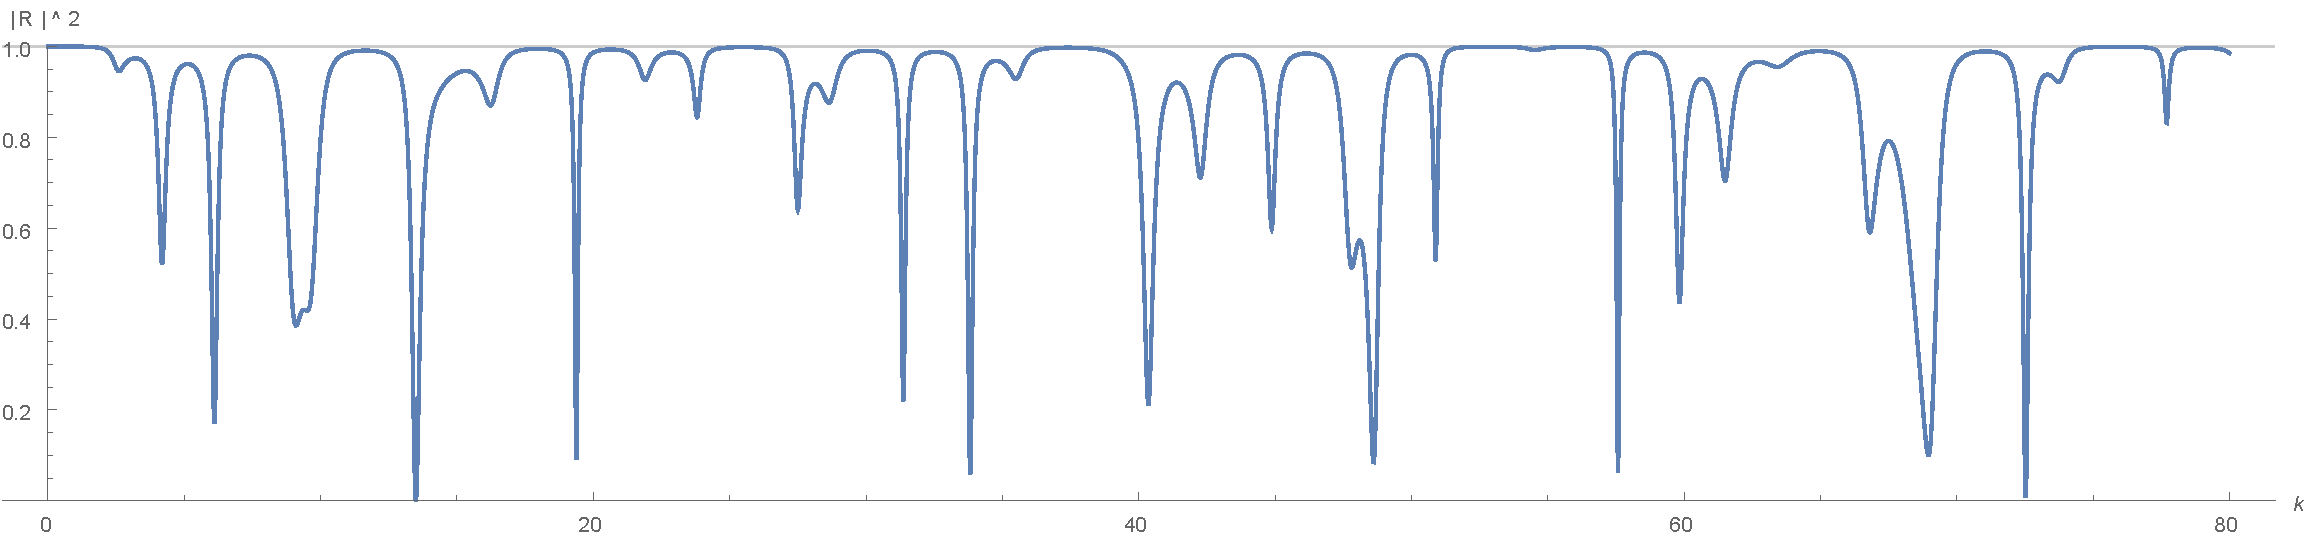
\includegraphics[width=1\textwidth]{img/reflection_n=6_m=5_l=1_b=07_kmax=80}
    \caption{$n=6, m=5, \ell_0=1, \beta=0.7$}
  \end{subfigure}
  \begin{subfigure}[t]{\textwidth}
    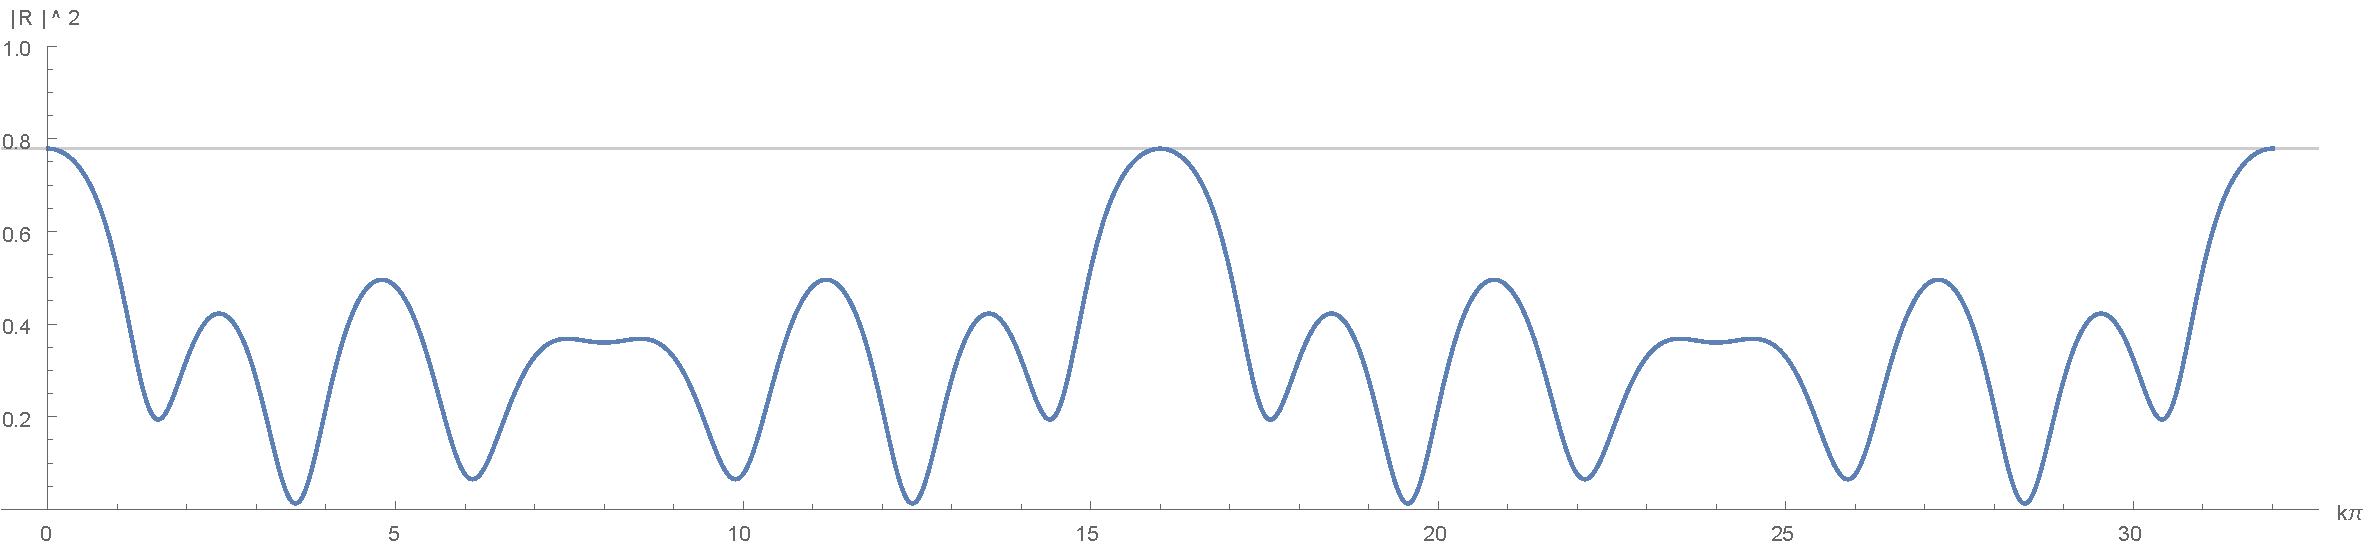
\includegraphics[width=1\textwidth]{img/reflection_n=4_m=2_l=1_b=05_kmax=32pi}
    \caption{$n=4, m=2, \ell_0=1, \beta=0.5$}
  \end{subfigure}
  \begin{subfigure}[t]{\textwidth}
    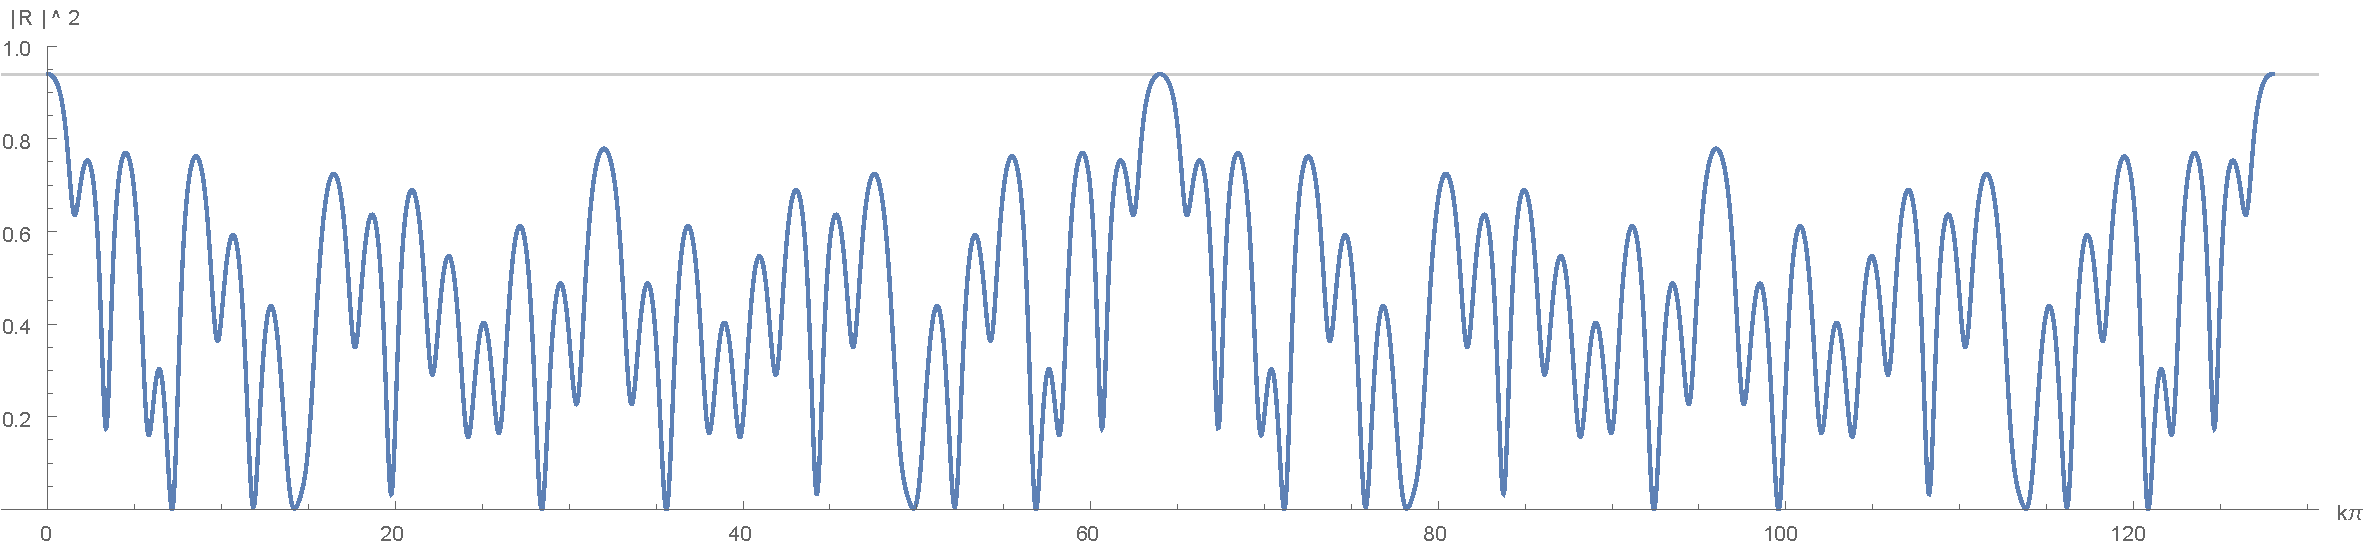
\includegraphics[width=1\textwidth]{img/reflection_n=6_m=2_l=1_b=05_kmax=128pi}
    \caption{$n=6, m=2, \ell_0=1, \beta=0.5$}
  \end{subfigure}
  \caption{Scattering from snowflakes with different parameters.}
  \label{fig: snowflake reflection graphs}
\end{figure}

\clearpage




\section{Band gap structure in the periodic snowflake}

We now consider the case $\beta = 1$, which is considerably easier to deal with since all phase factors in the expression for $S_{ll,n}(k)$ coincide. In particular this gives a periodic graph, all edges have the same length $\ell$.
% For clarity we will $R_n = S_{ll,n}$ and $T_n = S_{rl,n}$.

% We begin by noting that for $k_0 = (2j+1)\pi/(2\ell)$ with $j=0,1,2,\ldots$ we have $S_{ll,n}(k_0) = 0$ for even $n$ and $S_{ll,n}(k_0) = \frac{1-m}{1+m}$ for odd $n$. Indeed, $e^{2ik_0\ell} = -1$ and by equation \eqref{eq: recursion} we have
% \begin{align*}
%   S_{ll,2}(k_0)
%   &= S_{ll,1} + \frac{e^{2ik_0\ell} S_{rl,1} S_{ll,1} S_{lr,1}}{1 - e^{2ik_0\ell} S_{rr,1} S_{ll,1}} \\
%   &= S_{ll,1}\g{1 + \frac{e^{2ik_0\ell} S_{rl,1} S_{lr,1}}{1 - e^{2ik_0\ell} S_{rr,1} S_{ll,1}}} \\
%   &= S_{ll,1}\g{1 + \frac{e^{2ik_0\ell} S_{rl,1}^2}{1 + e^{2ik_0\ell} S_{ll,1}^2}} \\
%   &= S_{ll,1}\g{\frac{1 + e^{2ik_0\ell} \g{ S_{ll,1}^2 + S_{rl,1}^2}}{1 + e^{2ik_0\ell} S_{ll,1}^2}} \\
%   &= S_{ll,1}\g{\frac{1 - \g{ S_{ll,1}^2 + S_{rl,1}^2}}{1 - S_{ll,1}^2}} \\
%   &= 0,
% \end{align*}
% where we have used that $S_{ll,1}^2+S_{rl,1}^2 = 1$ since $S_{ll,1}$ and $S_{rl,1}$ are real an the wave is preserved after scattering. Next, this immediately gives $\abs{S_{rl,2}}^2 = 1$, hence

% Hence $S_{ll,n}(k_0) = 0$ for all $n \ge 2$. We have a similar result for total reflection.

We begin by making a simple observation

\begin{lemma}\label{res: maximal periodic reflection}
  Let $\Gamma$ be a periodic snowflake graph with $n$ generations and branching number $m$. Let $k_1 = j\pi/\ell$ for any integer $j$. The reflection from $\Gamma$ at energies $k_1$ is given by
  \begin{align*}
    S_{ll,n}(k_1) = \frac{1-m^n}{1+m^n}.
  \end{align*}
\end{lemma}
\begin{proof}
  From \cref{eq: recursion} we see that this holds for $n=1$. Note that $e^{2ik_1\ell} = 1$ and use that since all edge lengths are equal, the phases coincide, and we have $S_{ll,n}=-S_{rr,n}$ and $S_{rl,n} = S_{lr,n}$. Assume the result holds for $S_{ll,n}$, then
  \begin{align*}
    S_{ll,n+1}
    &= S_{ll,n} + \frac{e^{2ik\ell_n} S_{rl,n} S_{ll,1} S_{lr,n}}{1 - e^{2ik\ell_n} S_{rr,n} S_{ll,1}} \\
    &= S_{ll,n} + \frac{S_{rl,n}^2 S_{ll,1}}{1 + S_{ll,n} S_{ll,1}} \\
    &= \frac{S_{ll,n} + \g{S_{ll,n}^2 + S_{rl,n}^2} S_{ll,1}}{1 + S_{ll,n} S_{ll,1}} \\
    &= \frac{S_{ll,n} + S_{ll,1}}{1 + S_{ll,n} S_{ll,1}} \\
    &= \frac{\frac{1-m^n}{1+m^n} + \frac{1-m}{1+m}}{1 + \frac{1-m^n}{1+m^n} \frac{1-m}{1+m}} \\
    &= \frac{1-m^{n+1}}{1+m^{n+1}}.
  \end{align*}
  We also used that $S_{ll,1}^2+S_{rl,1}^2 = 1$ since $S_{ll,1}$ and $S_{rl,1}$ are real and the wave is preserved after scattering.
  The result follows by induction.
\end{proof}

\begin{corollary}\label{res: R(0)}
  Let $\Gamma$ be a quantum snowflake graph with $n$ generations and branching number $m$. The reflection of an incoming wave with zero energy from $\Gamma$ is given by
  \[
    S_{ll,n}(0) = \frac{1-m^n}{1+m^n} = \frac{2}{m^n+1} - 1,
  \]
  precisely that of a star graph with degree $m^n+1$. That is, for very low energies the incoming wave does not ``see'' the inner edges.
\end{corollary}
\begin{proof}
  \Cref{res: maximal periodic reflection} holds in particular for $k_1 = 0$. For this value of $k$ the lengths of the edges do not come into play and we can remove the requirement that the graph must be periodic.
\end{proof}


If we increase the number of generations, we see that the maximal reflection found in \cref{res: maximal periodic reflection} approaches 1. Indeed,
\[
  S_{ll,n}(k_1) = \frac{1-m^n}{1+m^n} = \frac{2}{m^n+1} - 1,
\]
and for $m \ge 2$ it is clear that $\abs{S_{ll,n}(k_1)}^2 \to 1$ as $n\to\infty$. In figure~\ref{fig: periodic snowflake reflection graphs} we plot the reflection from periodic snowflakes for varying generations. These plots indicate that there are intervals for which we get total reflection as $n\to\infty$. We shall investigate this further.

\begin{figure}[!h]
  \centering
  \begin{subfigure}[t]{0.8\textwidth}
    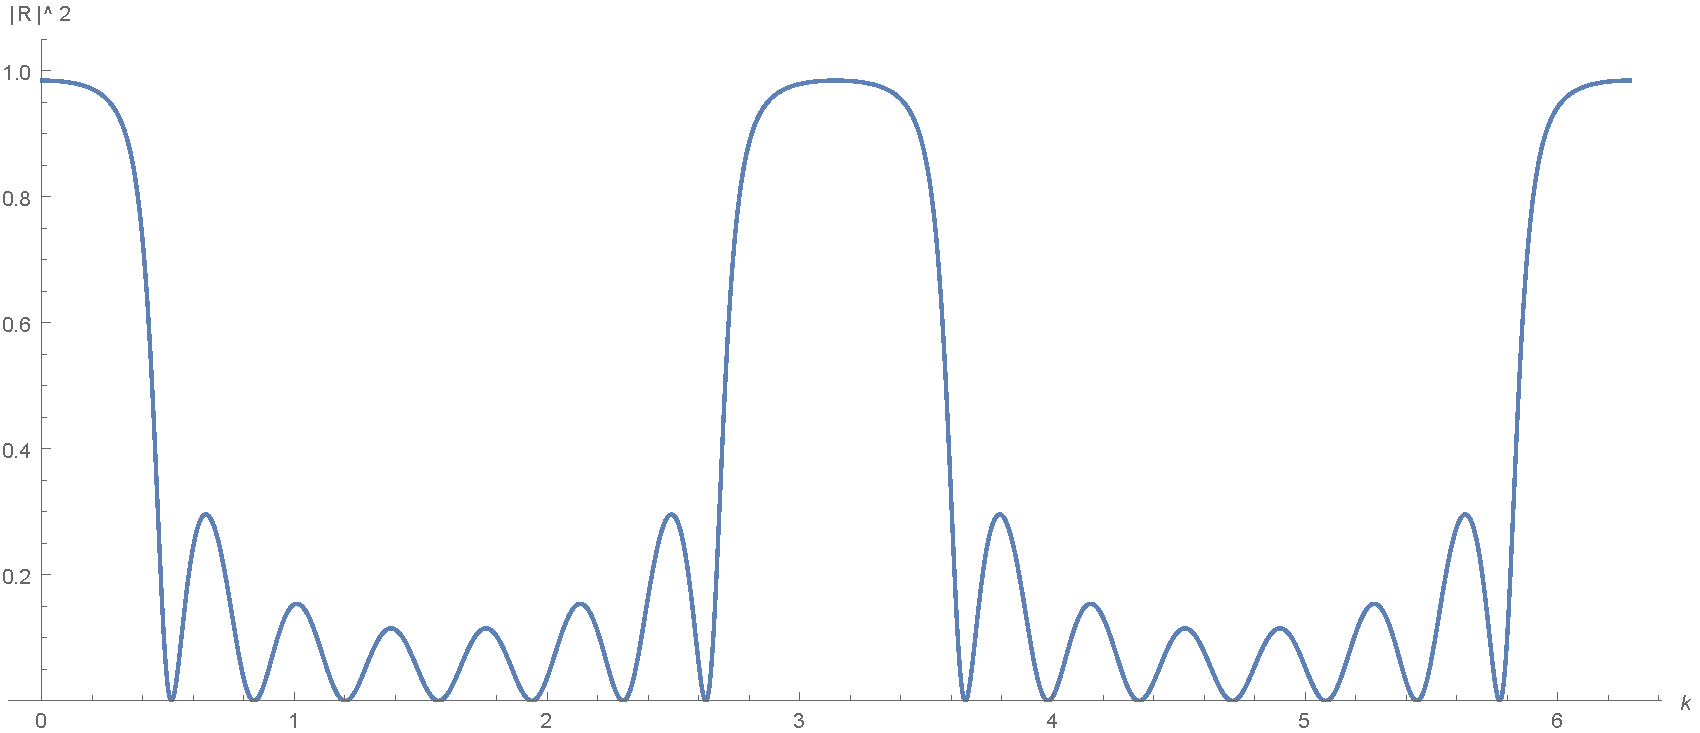
\includegraphics[width=\textwidth]{img/reflection_n=4_m=2_l=1_b=1_int=2pi}
    \caption{$n=8, m=2, \ell=1, \beta=1$}
  \end{subfigure}
  \begin{subfigure}[t]{0.8\textwidth}
    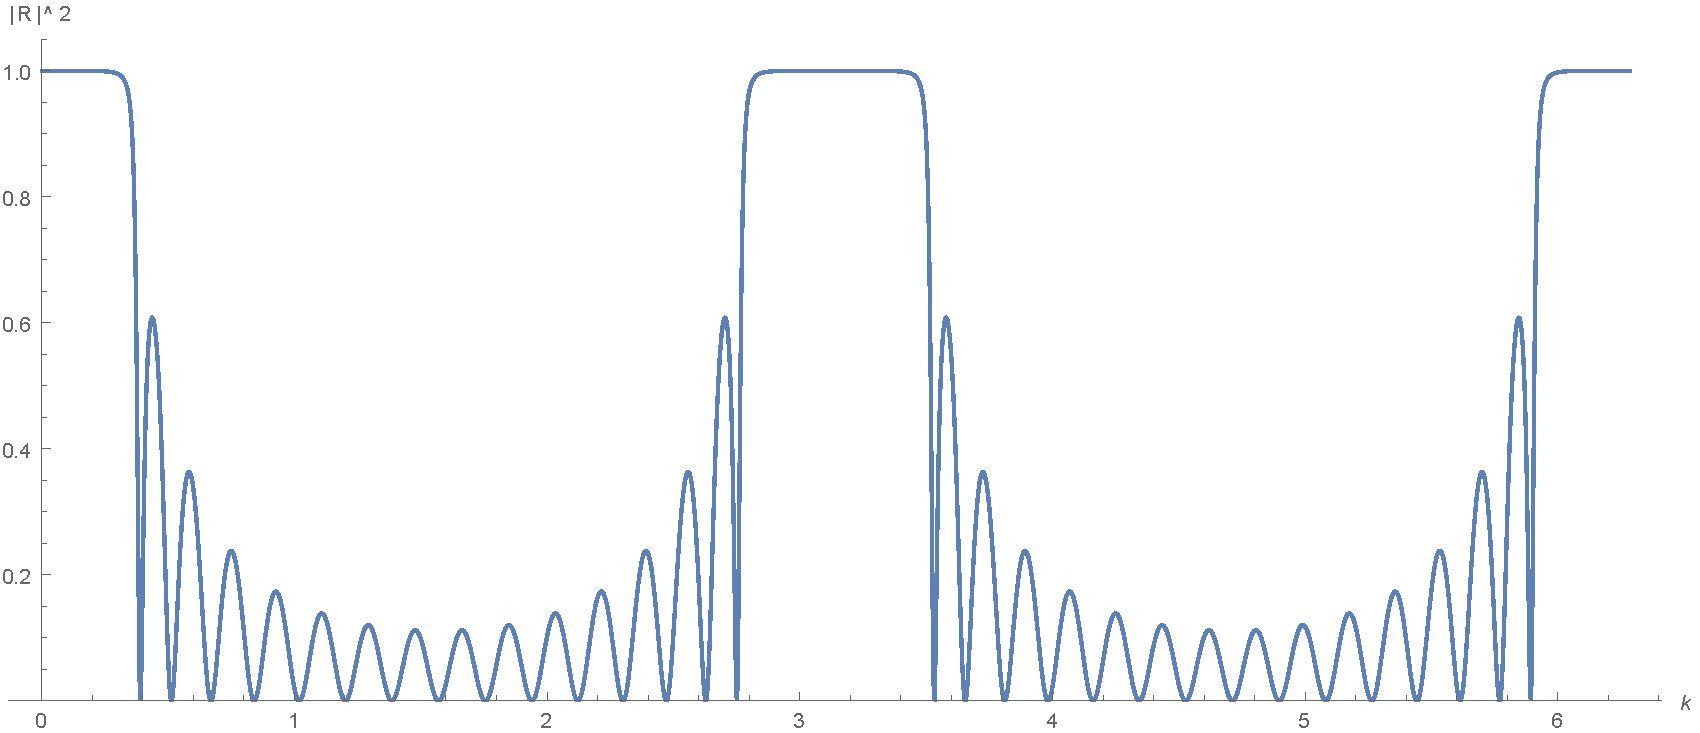
\includegraphics[width=\textwidth]{img/reflection_n=5_m=2_l=1_b=1_int=2pi}
    \caption{$n=16, m=2, \ell=1, \beta=1$}
  \end{subfigure}
  \begin{subfigure}[t]{0.8\textwidth}
    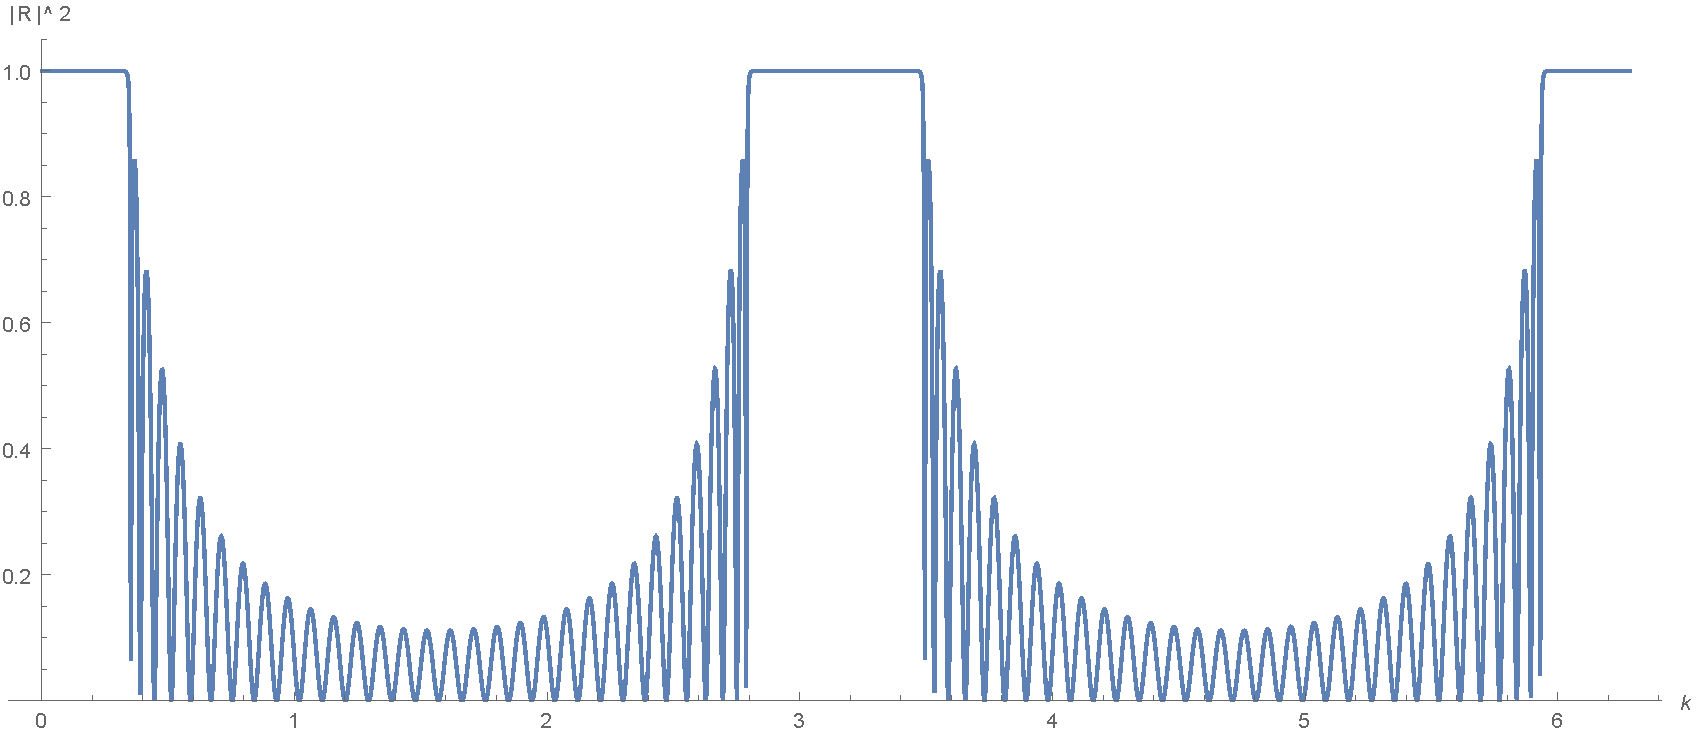
\includegraphics[width=\textwidth]{img/reflection_n=6_m=2_l=1_b=1_int=2pi}
    \caption{$n=32, m=2, \ell=1, \beta=1$}
  \end{subfigure}
  % \begin{subfigure}[t]{0.8\textwidth}
  %   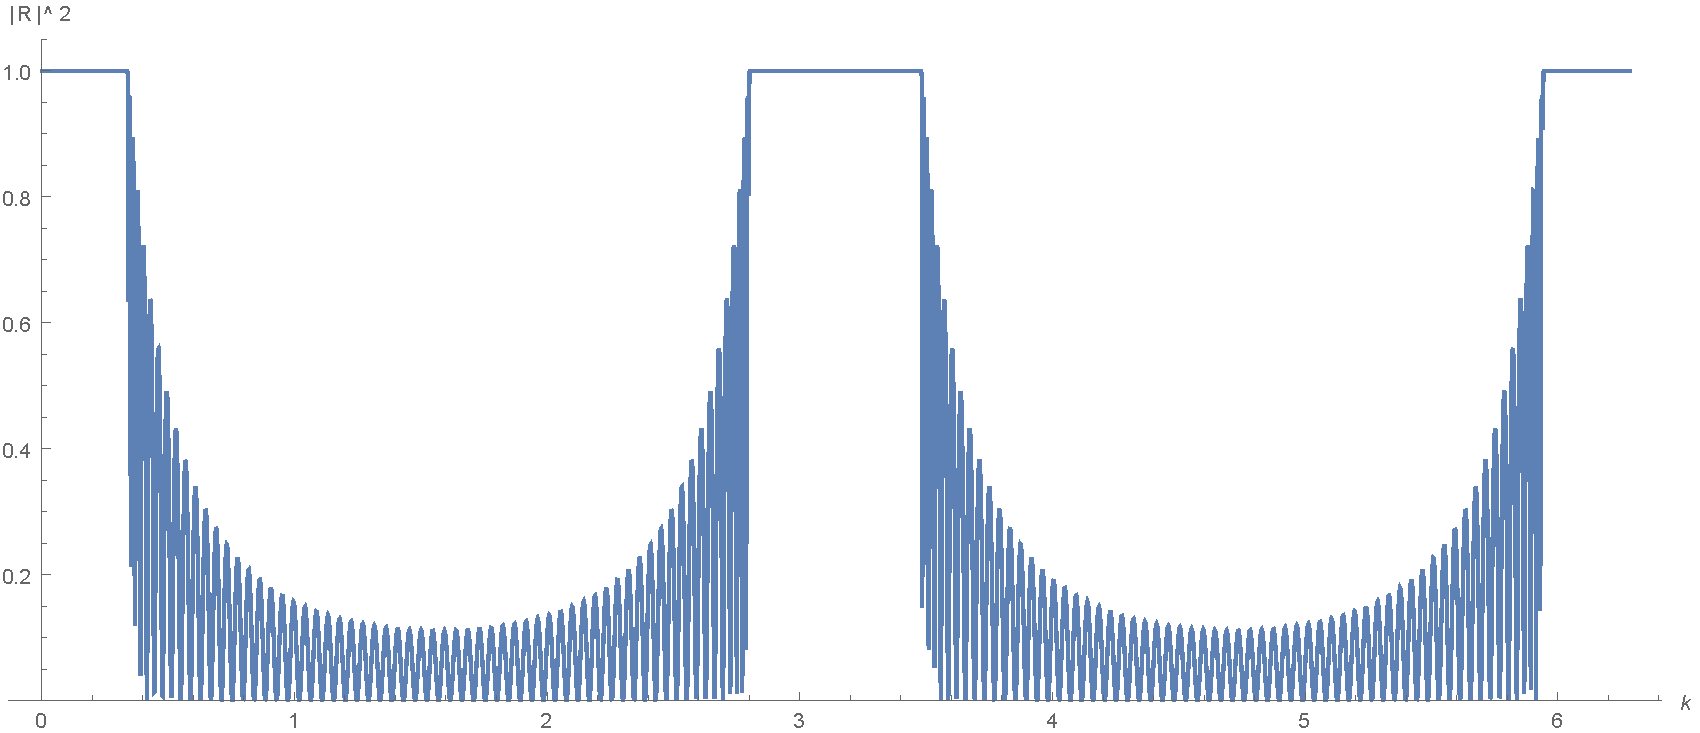
\includegraphics[width=\textwidth]{img/reflection_n=7_m=2_l=1_b=1_int=2pi}
  %   \caption{$n=64, m=2, \ell=1, \beta=1$}
  % \end{subfigure}
  \caption{Scattering from periodic snowflakes with increasing number of generations.}
  \label{fig: periodic snowflake reflection graphs}
\end{figure}
\clearpage

To capture the fact that the snowflake graph with $\beta=1$ and edge length $\ell$ is invariant under translation of distance $\ell$, we introduce the translation operator $T_\ell$ as translating a function on the graph by distance $\ell$: $(T_\ell f)(x) = f(x+\ell)$. Because of the self-similarity of the graph, the probability density of a particle described by eigenfunctions $f$ to $L$ must be the same at position $x$ and $x+\ell$. That is, we must have $\abs{f(x)}^2 = \abs{f(x+\ell)}^2$, implying that the function varies by at most a phase factor $e^{i\theta}$ from the point $x$ to $x+\ell$. Hence we have $(T_\ell f)(x) = f(x+\ell) = e^{i\theta} f(x)$. This result is more generally known as Bloch's theorem in solid state physics, and a function on the form $e^{i\theta} f(x)$ is called a Bloch wave.

Furthermore we see that $T_\ell$ commutes with $L = -\Dopn{x}{2}$, i.e.\ $T_\ell L = LT_\ell$, since the phase factor $e^{i\theta}$ does not affect the differentiation. Hence the eigenfunctions of both operators can be chosen equal, c.f.\ theorem~\ref{thm: commuting operators share eigenfunctions}.
Due to the self-similarity it is sufficient to consider only one edge of the graph, parametrize it from $0$ to $\ell$.

In section 4.1 in \cite{pavel book} the transfer matrix
\[
  T(\lambda, x_1, x_2) :
  \begin{pmatrix}
    f_\lambda(x_1) \\
    f_\lambda'(x_1)
  \end{pmatrix}
  \mapsto
  \begin{pmatrix}
    f_\lambda(x_2) \\
    f_\lambda'(x_2)
  \end{pmatrix}
\]
is introduced, where $f_\lambda$ is any solution to $Lf_\lambda = \lambda f_\lambda$ with the corresponding eigenvalue $\lambda$. This matrix maps Cauchy data for $x=x_1$ to Cauchy data for $x=x_2$ the edge. By Cauchy data we mean the vector containing the function value and the value of the derivative. Note that this is only valid when $x_1$ and $x_2$ are on the same edge, when passing over a vertex, one must take the matching conditions into consideration. The transfer matrix is given by
\[
  T(\lambda, x_1, x_2) =
  \begin{pmatrix}
    \cos k(x_2-x_1) & \dfrac{\sin k(x_2-x_1)}{k} \\
    -k \sin k(x_2-x_1) & \cos k(x_2-x_1)
  \end{pmatrix}, \quad k = \sqrt{\lambda}.
\]

Furthermore, from the snowflake matching conditions we have that the Cauchy data, as we pass over a vertex, is transformed by
\[
  \begin{pmatrix}
    f_\lambda(+0) \\
    f_\lambda'(+0)
  \end{pmatrix}
  =
  \begin{pmatrix}
    \sqrt{m} & 0 \\
    0 & 1/\sqrt{m}
  \end{pmatrix}
  \begin{pmatrix}
    f_\lambda(-0) \\
    f_\lambda'(-0)
  \end{pmatrix}.
\]
Combining this with the transfer matrix inside the edge at position $x=\ell-0$ gives
\begin{align*}
  \begin{pmatrix}
    f_\lambda(\ell-0) \\
    f_\lambda'(\ell-0)
  \end{pmatrix}
  &=
  \begin{pmatrix}
    \cos k\ell & \dfrac{\sin k\ell}{k} \\
    -k \sin k\ell & \cos k\ell
  \end{pmatrix}
  \begin{pmatrix}
    \sqrt{m} & 0 \\
    0 & 1/\sqrt{m}
  \end{pmatrix}
  \begin{pmatrix}
    f_\lambda(-0) \\
    f_\lambda'(-0)
  \end{pmatrix} \\
  &=
  \begin{pmatrix}
    \sqrt{m}\cos k\ell & \dfrac{\sin k\ell}{k\sqrt{m}} \\
    -k\sqrt{m} \sin k\ell & \dfrac{\cos k\ell}{\sqrt{m}}
  \end{pmatrix}
  \begin{pmatrix}
    f_\lambda(-0) \\
    f_\lambda'(-0)
  \end{pmatrix}.
\end{align*}
This is precisely a translation by distance $\ell$, hence we can use the translation operator $(T_\ell f)(-0) = f(\ell-0) = e^{i\theta} f(-0)$ and write the above equation as
\begin{align*}
  \begin{pmatrix}
    \sqrt{m}\cos k\ell & \dfrac{\sin k\ell}{k\sqrt{m}} \\
    -k\sqrt{m} \sin k\ell & \dfrac{\cos k\ell}{\sqrt{m}}
  \end{pmatrix}
  \begin{pmatrix}
    f_\lambda(-0) \\
    f_\lambda'(-0)
  \end{pmatrix}
  =
  e^{i\theta}
  \begin{pmatrix}
    f_\lambda(-0) \\
    f_\lambda'(-0)
  \end{pmatrix}.
\end{align*}
This shows that the matrix
\[
  A =
  \begin{pmatrix}
    \sqrt{m}\cos k\ell & \dfrac{\sin k\ell}{k\sqrt{m}} \\
    -k\sqrt{m} \sin k\ell & \dfrac{\cos k\ell}{\sqrt{m}}
  \end{pmatrix}
\]
has eigenvalue $e^{i\theta}$ --- recall that the eigenfunctions of $T$ and $L$ can be chosen to be equal. More generally, let $\lambda_1$ and $\lambda_2$ denote the eigenvalues of $A$. In general we have that the product of the eigenvalues of a matrix is given by its determinant and the sum of the eigenvalues is given by its trace. We clearly have $\det A = 1$ and let $t$ denote the trace $\Tr A$, thus we have
\[
  \left\lbrace\begin{aligned}
    \det A &= 1 = \lambda_1 \lambda_2 \\
    \Tr A &= t = \lambda_1 + \lambda_2.
  \end{aligned}\right.
\]
This system can be written as
\[
  \lambda_1^2 - t\lambda_1 + 1 = 0
\]
and has the solutions
\[
  \lambda_1 = \frac{t\pm\sqrt{t^2-4}}{2}.
\]
But we know that the eigenvalues are on the form $e^{i\theta}$, hence there exists a $\theta$ such that $\lambda_1 = e^{i\theta} = \cos \theta + i \sin \theta$. In particular $\lambda_1$ must have an imaginary component, this is only possible if
% \begin{gather*}
%   t = \g{\frac{1}{\sqrt{m}} + \sqrt{m}}\cos k\ell = 2 \cos \theta \\
%   \pm \sqrt{t^2-4} = i \sin \theta
% \end{gather*}
we have $t^2-4 < 0$, that is $-2 < t < 2$. Using that
\[
  t = \g{\sqrt{m}+\frac{1}{\sqrt{m}}}\cos kl = \g{\frac{1+m}{\sqrt{m}}} \cos kl
\]
is the trace of $A$, we get the condition
\[
  -2 < \g{\frac{1+m}{\sqrt{m}}} \cos kl < 2.
\]
Only the values for $k$ that satisfy the above inequality are realizable energies in the graph, hence we must have total reflection for waves approaching the graph with energies corresponding to values of $k$ that do not satisfy this inequality. We record this as a theorem.

\begin{theorem}[Band gap structure in the periodic snowflake graph]
  Let $\Gamma$ be a periodic quantum snowflake graph with edge lengths $\ell$ and branching number $m$. Only energies $\lambda = k^2$ satisfying
  \[
    \abs{\cos k\ell} < \frac{2\sqrt{m}}{m+1}
  \]
  are realizable in the graph. Incoming waves with energies not satisfying this inequality are totally reflected.
\end{theorem}

In figure~\ref{fig: periodic snowflake reflection band gap} the reflection of a periodic snowflake is plotted along with $\frac{m+1}{2\sqrt{m}} \abs{\cos k\ell}$ to clearly show how the band gap structure of the graph emerges already for a low number of generations.


\begin{figure}[!h]
  \centering
  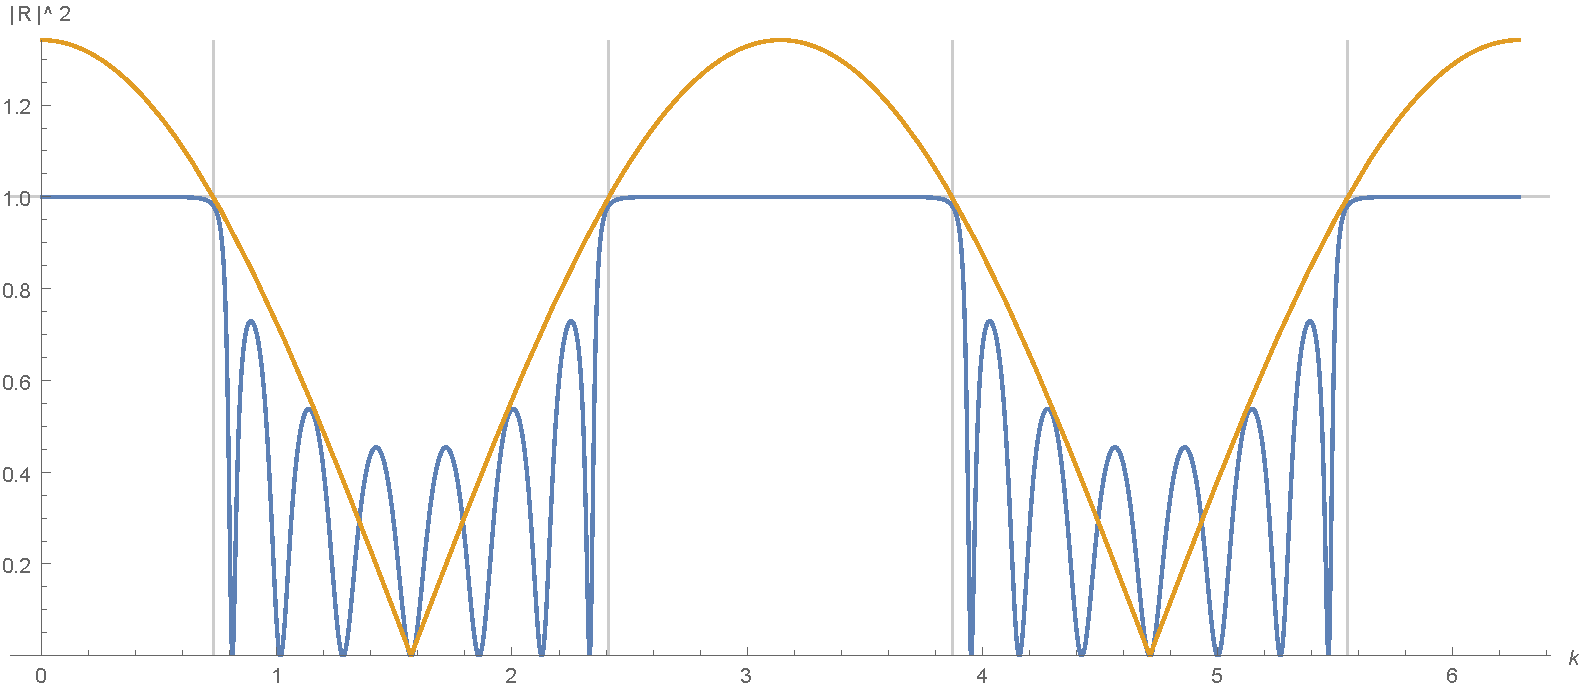
\includegraphics[width=\textwidth]{img/reflection_n=4_m=5_l=1_b=1_int=2pi_bandgap}
  \caption{Band gap structure for a quantum snowflake graph with parameters $n=8, m=5, \ell=1$.}
  \label{fig: periodic snowflake reflection band gap}
\end{figure}

% Based on the same method we can analyze the values of $k$ for which zero reflection is obtained.

It is interesting to study not only how the reflection depends on the energy, but also the average reflection over a period of $\abs{R}^2$, which for the periodic snowflake takes the simple form:
\[
  \frac{1}{2\pi\ell} \int_{0}^{2\pi\ell} \abs{R(k)}^2 dk = \frac{m-1}{m+1}
\]
where $m$ is the branching number.
This integral is not straight forward to calculate analytically. The stated value of the integral was obtained by numerical integration using a high number $n$ of generations and several different values for $m$, the closed-form expression $\frac{m-1}{m+1}$ is an extrapolation. Observe that $\frac{m-1}{m+1} = \abs{S_{ll,1}(0)}$, i.e.\ the average reflection from the periodic snowflake graph is the square root of the (constant) reflection from the star graph of degree $m+1$.

% Studying the average reflection for various configurations of snowflake graphs is one of several properties that could be further studied.
% The case $\beta = 1/2$ reveals no such relations for $m=2$ fixed with increasing number of generations, after numerically studying the integral over the period of $\abs{R}^2$.



% \section{\texttt{work in progress}}

% Consider a snowflake graph with the wavefunction on edge $e_0$ given by $e^{ikx} + R(\ell_0)$ and on $e_1$ given by $Ae^{ikx} + Be^{-ikx}$. Consider the snowflake graph given by removing edge $e_0$, letting edge $e_1$ play the role of the root edge, of length $\ell_0\beta$. For this graph, the resulting reflection can be written as $R(\ell_0\beta) = B/A$, that is, the wavefunction on the root edge is given by $A(1+R(\ell_0\beta))$.

% The matching conditions \eqref{eq: snowflake mc} at $v_1$ in the original graph can thus be written as
% \begin{equation*}
%   \left\lbrace\!\!
%   \begin{aligned}
%     e^{ik\ell_0} + R(\ell_0)e^{-ik\ell_0} &= \frac{A+B}{\sqrt{m}} = A \frac{1+R(\ell_0\beta)}{\sqrt{m}} \\
%     e^{ik\ell_0} - R(\ell_0)e^{-ik\ell_0} &= \sqrt{m}(A-B) = A\sqrt{m} (1+R(\ell_0\beta)).
%   \end{aligned}
%   \right.
% \end{equation*}
% Dividing the first equation by the second equation gives
% \begin{align*}
%   \frac{e^{ik\ell_0} + R(\ell_0)e^{-ik\ell_0}}{e^{ik\ell_0} - R(\ell_0)e^{-ik\ell_0}} = \frac{1+R(\ell_0\beta)}{m(1-R(\ell_0\beta))}.
% \end{align*}
% Solving for for $R(\ell_0\beta)$
% \[
%   R(\ell_0\beta) = \frac{(m-1)e^{2ik\ell_0} + (m+1)R(\ell_0)}{(m+1)e^{2ik\ell_0}+(m-1)R(\ell_0)}
% \]
% and solving for $R(\ell_0)$
% \[
%   R(\ell_0) = e^{2ik\ell_0} \frac{(1-m) + (1+m)R(\ell_0\beta)}{(1 + m) + (1-m)R(\ell_0\beta)}.
% \]
% Compare this to \eqref{eq: scattering coefficients 2 generation snowflake} or \eqref{eq: recursive Rn} which gives
% \[
%   R_2 = \frac{(1-m)+(1+m)R_1e^{2ik\ell_1}}{(1+m)+(1-m)R_1e^{2ik\ell_1}}
% \]

% There's something fishy with the phases when comparing the last two equations. Also, does this method give anything more than what was found in the previous subsection?
